\documentclass
[
	12pt,
	a4paper,
	oneside,
	openany,
%	titlepage
]{report}
%titlepage prints the title on it's own page in article class

% Use a different font -commented out for cloud 9 compatibility
% Doesn't automatically change font for math mode so commented out
%\usepackage{times}

\usepackage[utf8]{inputenc}
\pagestyle{myheadings}
\markright{Gregory Cartwright --- 3403548}

% 1.5 space my text
\renewcommand{\baselinestretch}{1.5}

%reduce the hyphenation of words
\sloppy

%prints a small space between paragraphs and removes the indenting of the first line
\setlength{\parskip}{2ex plus0.5ex minus 0.2ex}
\setlength{\parindent}{0em}

%csquotes - provides multilingual quoting - keeps babel happy
\usepackage{csquotes}
%babel required for biblatex to work. Specifying british last make it the language in use
%\usepackage[english,british]{babel}
\usepackage[british]{babel}

\usepackage[style=authoryear,backend=biber,
	giveninits=true,
	dateabbrev=false,
	uniquename=init,
	citestyle=authoryear,
	dashed=false,
	maxcitenames=2,
	maxbibnames=99,
	sorting=nyt,
	language=british]{biblatex}

% Remove "In:" form before name of journal
\renewbibmacro{in:}{%
	\ifentrytype{article}{}{\printtext{\bibstring{in}\intitlepunct}}}

%Add a comma between name and year in citations
\renewcommand*{\nameyeardelim}{\addcomma\space}
%put double space between entries in the references
\setlength\bibitemsep{2\itemsep}

%remove hanging indent from the reference list
\setlength\bibhang{0em}

%Ensure all names in reference list are formatted as Surname, I.
\DeclareNameAlias{default}{last-first}
\DeclareNameAlias{sortname}{last-first}

%Code to format journal article volume and issue as v (i)
\renewbibmacro*{volume+number+eid}{
	\printfield{volume}
	\setunit*{\addnbspace}
	\printfield{number}
	\setunit{\addcomma\space}
	\printfield{eid}
}
\DeclareFieldFormat[article]{number}{\mkbibparens{#1}}

%Code to format the 'Accessed day month year' in the references
\DeclareFieldFormat{urldate}{%
	[Accessed \thefield{urlday}\addspace%
  \mkbibmonth{\thefield{urlmonth}}\addspace%
  \thefield{urlyear}]}
  
%Code to format the 'Available from:' in the URL in references
\DeclareFieldFormat{url}{\bibstring{urlfrom}\addcolon\space\url{#1}}
\DefineBibliographyStrings{british}{
	urlfrom = {Available from}
}

%Command to STOP the references section and everything after having it's own header.
% The first for reports, second for articles
\defbibheading{bibintoc}[\refname]{\chapter{#1}}
%\defbibheading{bibliography}[\refname]{\section*{#1}}

\usepackage{graphicx}

% package changepage contains adjustwidth environment used by the
% titlepage
\usepackage{changepage}

% Add my bibliography file here
\addbibresource{references.bib}

\begin{document}

%\author{Gregory Cartwright\\
%	Student number 3403548\\
%	MSc Advanced Nurse Practitioner dissertation
%}
%\title{Does level of frailty influence advance care planning 
%	for community hospital inpatients?
%}

%\maketitle

\begin{titlepage}

\begin{center}
	{\huge Does level of frailty influence advance care planning 
	for community hospital inpatients?}
\end{center}
	\vspace{4cm}
\begin{adjustwidth}{3cm}{}
	{\large A dissertation submitted in partial fulfilment of the 
	requirements for the MSc Advanced Nurse Practitioner.}
\end{adjustwidth}
	\vspace{2cm}
\begin{adjustwidth}{5cm}{}
Gregory Cartwright

School of Health and Social Care

London South Bank University

	{\textbf May 2018}
\end{adjustwidth}

\end{titlepage}

\begin{abstract}
The population of the United Kingdom is
ageing and with this the prevalence of frailty is increasing. National 
guidance suggests that the presence of frailty in a person should trigger,
amongst other things, consideration of advance care planning. The aim of this
is to ensure that they get the most appropriate treatment in this phase of
their life.

Patients in the local community hospitals are likely to be quite frail and
few have advance care plans when they arrive. Some patients undergo
advance care planning during their community hospital stay, but most do not.
This can mean that when their health 
deteriorates they may get admitted to the Emergency Department when the 
outcome of this might actually be detrimental to them.

This study examines if the level of frailty 
	of these patients influences whether or not they get advance 
	care planning during their hospital stay and what other factors,
	age, gender and presenting complaint, might influence this process.

	To achieve this aim a retrospective observational cross-sectional
	study was designed. A sample of 148 recently discharged 
	community hospital patients were conveniently sampled. The case notes
	of these were reviewed to assess the level of frailty with the
	Clinical Frailty Scale, and whether
	they had a preexisting advance care plan prior to admission.

	The notes of those patients who did not have a preexisting advance 
	care plan were then further examined to see if advance care planning
	was considered during their stay and to gather information on their
	age, gender and presenting compliant. This data was then analysed
	to look for associations between advance care planning and frailty
	and the other variables.
	
	The findings were that 94 patients (63.5\%) had either moderate 
	or severe frailty.  Only 6 patients (4.1\%) had a 
	preexisting advance care plan. 
	Advance care planning was associated with frailty ($p=0.007$), 
	age ($p=0.016$) and
	presenting complaint ($p=0.034$). It is not clear what influence
	each of these factors had on the decision making process around 
	advance care planning, or how they interact with each other.

	The study recommends that severe frailty should be used as a 
	trigger to consider advance care planning for community hospital
	inpatients. It is also recommended that further research
	is needed to examine the links between frailty and the presenting
	complaints of patients to look into frailty syndromes, and to 
	explore the decision making around advance care planning. Hopefully
	this would help refine the criteria that prompts advance care 
	planning for these patients.
	
\end{abstract}

\section*{Acknowledgements}
\setcounter{page}{3}
The author would like to thank his wife Victoria and his children Bertie and
Bea for their patience and support whilst working on this dissertation.
He would like to thank his supervisor, Sharon, for her advice and assistance.
The following people also need to be thanked as they have provided help in
one way or another which is much appreciated: 
Caroline Barclay,
Dan Spence,
Graeme Pettifer,
Jonny Dexter,
Karen Plowman,
Kaye Hepple,
Lisa Shirkie,
Lynn MacDiarmid,
Mandy Cooper,
Ruth Tandy,
Sarah Boldy,
Simon Conroy.

\tableofcontents 
\listoftables
\listoffigures

\chapter{Introduction}

\section{Background}

\subsection{Population factors}

Over recent decades 
improvements in lifestyle and developments in medicine and healthcare have led
to people living longer \parencite{nao:08,ons:17}. Subsequently the population 
of the United Kingdom (UK) is getting older and this trend is forecast 
to continue.
In 2016 18\% of the population was over 65 years old. This is expected to be
23.9\% by 2036 \parencite{ons:17}.

People are living longer but with increasing morbidity. The older people are, 
the more
likely they are to have multiple chronic diseases. In a large scale study in
Scotland, \textcite{barnett:12} found that the percentage of the population with 
multimorbidity was around 
65\% in those aged 65 to 84, rising to 81\% in those aged 85 or over. A simulation 
to project multimorbidity over the next 20 years found that the number of people
aged 65 or over that have two or more diseases is likely to increase by 86\% and 
those with four or more disease is forecast to increase by 157\%
\parencite{kingston:18}. 

\subsection{Introducing frailty}

Multimorbidity is linked to frailty which can be viewed as a state where 
the function and resilience of multiple body systems is impaired \parencite{woo:14}. 
The prevalence of frailty is therefore likely to increase with multimorbidity 
as the population
gets older \parencite{sharp:13}. Indeed, a review of all hospital admissions in 
England found an increase in inpatient frailty over an eight year period 
\parencite{soong:15}.

There are varying definitions of frailty \parencite{soong:15}, however there is 
agreement that it is a condition where the maintenance of homeostasis 
becomes vulnerable to small stressors \parencite{vellas:16}. Examples of such 
stressors which would be trivial for people who are fit, include changes in 
environment and minor illness. The consequences in frailty of 
exposure to these are wide ranging and include delirium, significant reduction 
in mobility, falls, increased dependency, non-specific failure to thrive and death 
\parencite{bgs:14,oliver:14,vellas:16}.

\subsection{Implications of frailty}

A person with frailty who becomes ill is therefore exposed to many risks. If
they are subsequently admitted to an acute hospital then the  
change in environment becomes an additional stressor, further increasing the 
likelihood of them developing
new problems. Indeed, frailty combined with acute illness carries a high risk 
of death.

Frailty is known as the biggest cause of mortality in older people 
\parencite{gill:10}. As a person becomes increasingly frail, they move towards 
the end of life, even 
though they do not have a definitive terminal diagnosis. This transition is
often not recognised by the healthcare team, possibly because it is a gradual process
compared to something like cancer entering a terminal phase when all curative
options are exhausted \parencite{oliver:14}. Dying with frailty is common.
Frail older people who have no terminal diagnosis account for about 40\% of 
deaths and only a quarter of deaths are from malignant disease \parencite{sharp:13}.

\subsection{Risks and benefits}
\label{sec:risk-ben}

\textcite{beauchampChildress:01} postulate four principles of healthcare, two
of which are beneficence and nonmaleficence.
When making decisions on how to proceed with a patient's care and treatment
it is therefore necessary to establish what the likely benefits and possible 
harms are from the proposed actions. It is also necessary to gain an insight 
into the likelihood of these benefits and harms, given the overall situation that
the patient is in at this time. This requires both a knowledge of the patient's 
current illness and a good understanding of their history.

When a person is in this phase, the likely benefits of acute admission are small.
The risks involved with admitting a person in this situation
to hospital are great.  
Indeed admission to acute hospital for people with frailty is associated with
poor outcomes including death \parencite{silver:12, wallis:15}. Risks and 
benefits have to be assessed and 
weighed up and sometimes the risks of such an undertaking actually
outweigh the intended benefits. The best outcome for the patient can be that 
they are not admitted. 

Decision making around this situation is complex 
The patient is often not able to contribute to this process because of changes 
in their
mental capacity due to delirium. If the assessing clinician does not know the 
patient and their situation and history, then this decision making is even more 
difficult. Often in such situations clinicians consider that the safest option is to 
admit the patient to an acute setting.

This is set against the year on year increase in the number of emergency hospital 
admissions in England, predominantly consisting of older people. Multiple 
national initiatives are in place to combat this \parencite{nao:18}.

\subsection{Advance Care Planning}

If declining condition due to frailty can be identified then discussions with the 
patient and their family can be had whilst they are not acutely unwell. These 
discussions should include what is important to the patient at this stage of their
life and plans can be made as to what should be done in particular circumstances
if their health deteriorates. This is known as advance care planning
(ACP) \parencite{jennings:18}. People often involve their spouse or other close 
relative in these discussions. If the person lacks capacity to make such
decisions, due to dementia for example, then advance care planning can still
happen. In these circumstances decision making has to be made in the best
interest of the person \parencite{ncpc:11}.

If an advance care plan is in place when a person becomes acutely unwell then it
can guide the decision making process for the clinician so that the most appropriate
action can be taken at that time, taking into account plans that have been made 
at a time when the person's health was more stable. This hopefully produces an
outcome for the patient and their family that is least risky, least distressing
and most in line with the patients wishes. In a randomised controlled trial
\textcite{detering:10} found that 86\% of patients who got ACP had their wishes
fulfilled at the end of life compared with 30\% of those who didn't get ACP.

This sounds ideal, however the \textcite{silver:12} reports that end of life care 
in older people with frailty
is something that is often not adequately considered. It has been suggested that 
end of life care services in the UK are aimed at those with malignant 
disease \parencite{sharp:13}, furthermore it seems that people with frailty 
are often not involved in planning their 
end of life care \textcite{oliver:14}. This is partly due to the aforementioned 
assertion 
that, in this group, entering an end of life phase is frequently not recognised 
\textcite{wallington:16} and
estimating prognosis is more problematic \parencite{silver:12}. However national
guidelines state that all care providers should identify people approaching 
the end of life and offer such people a care plan \parencite{dh:09}.
Frailty should be considered at the centre of older people's healthcare to guide
evidence based treatment \parencite{woo:14}.

\section{Local context}

\subsection{Practice environment}
\label{sec:local-practice}
The author is an advanced nurse practitioner (ANP) in a community Trust.
The Trust has eight community hospitals (CHs) which have twelve inpatient 
wards between them. Each ward has
an ANP who works on the ward to provide medical management of the patients during 
the hours of Monday to Friday, 0900 to 1730. The ANP is supported by a consultant
geriatrician or stroke physician who visits twice a week. Outside the hours of 
Monday to Friday, 0900 to 1730, medical care 
is provided by the out of hours (OOH) general practitioner (GP) service. 

Most patients are admitted to the community hospital for either rehabilitation
or medical step-down. The majority of these patients come following an acute admission
where they have been stabilised medically but are often deconditioned as a result
of acute illness and are not ready to go home. At this stage their needs include 
ongoing medical treatment and monitoring and further assessments and treatment such 
as physiotherapy and occupational therapy to prepare them for discharge home.

Some patients are admitted directly from home because they have medical or rehabilitation
needs that cannot be met at home but don't require an admission to an acute hospital.
A minority of patients are admitted for palliative care.

When patients are admitted to one of these wards they have a comprehensive geriatric 
assessment (CGA) \parencite{bgs:14}. This is a multi-faceted diagnostic process
performed by the multi-disciplinary team (MDT) to produce a plan for treatment 
and follow-up.
An international meta-analysis found that, when compared with general medical care,
CGA was effective at keeping older people alive and living in their own homes at
twelve months post admission with a number needed to treat of 33 \parencite{ellis:11}.

\subsection{Local frailty}

The author expects that many of the patients admitted to the wards have frailty.
The extent of this is not known, however the patients are generally old.
During the last financial year the
average age was 81 and 49\% of patients admitted were aged 85 or over. Many have 
care needs as seen above.

Although the patients are usually clinically stable when they arrive on the ward,
their condition can deteriorate. This is usually managed in the community hospital
ward environment. The patients can have investigations including blood tests, plain
x-rays and electrocardiograms (ECG) usually without leaving the community hospital.
They can also receive treatments such as intravenous (IV) fluids, IV antibiotics
and even blood transfusions.

There are times when a patient's health deteriorates such that optimum 
management of their
acute condition can only be delivered in an acute inpatient setting. This is when 
the sort of decision making discussed in Section~\ref{sec:risk-ben} has
to be tackled. The situation that the patient is in has to be evaluated. The 
expected benefits of a proposed acute admission have to be ascertained for the
individual patient and these need to be balanced against the risks posed by a transfer
to an acute setting for that person in that situation. There are many factors that 
will influence this process. Some of these will not be immediately obvious to a 
clinician who is meeting the patient for the first time.

When a patient deteriorates during the OOH period they will be reviewed by a clinician
from the OOH GP service. This practitioner will be unlikely to know the patient,
the situation they are in and what their priorities in life are. As the patient is
acutely unwell at this point they may be unable to engage in objective and measured
discussions about how their care should proceed at this point. The water may be
further muddied if the OOH GP is not fully aware of the capabilities of the 
community hospital. 

In an audit of acute hospital admissions from community hospital settings,
\textcite{endacott:15} found that 55\% of these admissions happened OOH. 
At this time the reviewing clinician only has a partial picture of the 
patient's situation. They are often unaware that patients are nearing the end
of life \parencite{brettell:18}. consequently it may 
be that they often will err on the side of caution and
admit patients to the acute setting when this course of action may not actually have
been in the best interest of the patient. Locally, this is reinforced by 
retrospective reviews
of all acute admissions of community hospital inpatients that are carried out by the 
ANP team. These often find that the admission could have been avoided. In the case
of particularly frail patients, the ANPs sometimes feel that transferring that
patient to the acute sector was probably not in the best interest of the patient. 
They then feel that they should have engaged that patient in advance care planning
earlier in their stay to limit inappropriate, unhelpful and possibly detrimental 
escalation of their care to an acute setting.

\section{Research focus}

\subsection{Clarifying the problem}

There are patients in community hospital beds whose health deteriorates during
the OOH hours period. Some of these patients are very frail and because advance
care planning has not been undertaken with them they get transferred to an acute 
hospital when the net benefit of this to the patient is likely to be negative.
Some patients in the community hospital wards do have such advance care planning 
carried out and subsequently, when some of them suffer an acute deterioration in
their health, they avoid being transferred. This ensures a more
dignified outcome for them, eliminating the risk and distress of the emergency
department (ED). Many of them recover.

Reducing the number of patients who get admitted to the ED would
also help to reduce the strain on that department. Ultimately this would be of
benefit to the local health economy.

National guidance states that community hospitals should offer advance care
planning to patients nearing the end of life \parencite{dh:09}.
Currently there is no formal criteria locally as to which patients get advance 
care planning.
The decision to commence this process is made subjectively, based on assessment 
by the ANP or consultant. Most of these patients are likely to be old or frail
or both. The proportion of local patients who get advance care planning is not known,
but the systematic review conduced by \textcite{sharp:13} found that most older
people wanted to have such discussions, with some patients believing that it 
should be a routine component of their care.  
It seems therefore that advance care planning should be happening more in community
hospitals, and that frailty could be a suitable trigger for this.

\subsection{Research in this area}

A quick literature search shows that there is a paucity of literature looking 
into frailty scoring in community hospitals.
A search of the London South Bank University (LSBU) library journals 
collection for ``community hospital frailty''
did not find any articles examining any factor that could prompt ACP.

Changing the focus of the search terms to ``frailty advance care planning''
was more fruitful.
An intervention to involve care home residents and community hospital patients
had a large uptake with more than half the participants taking up the option of
advance care planning that was offered to them \parencite{mcglade:17}. This 
study did not select people for ACP but offered it to all, however, given the 
setting of long term care, it can be assumed that the prevalence of frailty
amongst the participants was high. This study supports the assertion that many
older people with frailty would welcome ACP.

Whilst exploring avoidable admissions to acute hospital, \textcite{mytton:12} 
suggest that avoiding unnecessary admission depends on good decision making at 
the time. This is difficult when the person assessing the patient does not know
them or their history. If we can prompt more consideration of ACP then this 
should assist with informing the decision making process at the time of 
deterioration.  
The \textcite{bgs:14} advise that frailty should be used as a prompt to
commence individualised planning of future care. This should include plans
for urgent and emergency situations.

This project aims to look at the link between the patient cohort in the CH
being open to ACP, frailty being an adverse prognostic factor in acute illness 
and
ACP being explored with appropriate patients to ensure that, in urgent and 
emergency situations, the patient gets what is best for them.

\section{Overall research aim and individual objectives}

The overall aim of this study is to examine if there is a relationship 
between the 
level of frailty of community hospital in-patients and whether advance care planning
happens and what other factors might influence this process.

It has been seen that patients with frailty should be identified and this 
information should be used by clinicians to explore advance care planning with 
them.
This should subsequently help prevent unplanned acute admissions that are 
unlikely to be of benefit to the patient and are likely to cause them distress 
and harm.

The level of frailty amongst the patient cohort in the local CH is not currently
known. Some of these patients undergo ACP during their stay, but what 
influences when this is done is not explicitly known. Frailty may be a factor
in this decision making process, but it is likely that there are patient 
related elements that are also influential.

% ***** objectives
Therefore the objectives of this study are to:
\begin{enumerate}
\item	Ascertain the different levels of frailty within the local 
		community hospital population, and within these levels identify 
		how many do not have an ACP before admission.\label{obj:prevalence}
\item	Determine which factors, namely frailty score, age, gender and
		presenting complaint, influence whether or not an ACP is 
		completed during the inpatient stay.\label{obj:association}
\item	Formulate local recommendations for practice to help reduce unhelpful
		acute hospital admissions for people with frailty through more 
		effective preemptive planning of treatment escalation.
		\label{obj:recommend}
\end{enumerate}
% ***** objectives

Objective~\ref{obj:prevalence} will provide an insight into the demographics
of the patient cohort. Given that frailty should prompt consideration of ACP
it will provide information about the proportion of the patient population in
whom this should be considered. Patients who have an ACP prior to their admission
have already been through the ACP process, and it is assumed that the ACP will be 
noted by the CH team and translated into an appropriate plan for their CH stay.
With these patients it is therefore not appropriate to consider what factors 
influence ACP as it has already been undertaken, so these patients will not
be considered in the work for objective~\ref{obj:association}.

Some patients have advance care planning whilst they are in the
community hospital, but what prompts the team to
consider it for some patients and not for others is not known.
Objective~\ref{obj:association} will explore this question by examining the CH
journey of those patients 
who arrive there without an ACP. It will look at the facets of age, frailty, 
gender and presenting complaint in an attempt to see whether any of these are
influential factors in the process of deciding whether ACP
will be considered by the team for that patient.

The results of this exploration will be discussed along with the guidance that 
identification of frailty should prompt consideration of ACP and the knowledge
that many older people with frailty welcome such a process. This will lead to 
recommendations for CH clinicians to help them identify 
patients who will benefit from discussion about their future care at a time 
when their health is relatively stable.

\chapter{Literature review}

\section{Introduction}

This literature review will firstly look to establish what frailty is, how it
manifests and explore strategies that exist to assess frailty. With this 
background knowledge the research objectives can be tackled. 
Objective~\ref{obj:prevalence} relates to the prevalence of frailty in the
local CH population. Therefore the incidence of frailty at an international
and national level will be examined to give the reader an idea of what the
size of the issue of frailty is locally.

To understand the need for advance care planning in the context of frailty,
the consequences of frailty will be explored with a particular focus on the
combination of frailty and acute illness or acute deterioration in health. 
It is situations such as this which has been identified as a problem area
in the local CH.

The question of how to address and manage frailty will be considered. In 
particular the focus will be on what is recommended in the literature as 
strategies for determining the factors, in frailty, that can help to prompt
ACP in an effort to inform the reader about the background for research 
objective~\ref{obj:association}. The driving force behind that objective 
is the benefits of ACP for people with 
frailty, therefore the proposed and observed boons of ACP will be briefly 
visited.

It is hoped that this will provide a good background to the area of research
and the intent is that a rationale for the need for this study will be 
exhibited. To clarify the situation, a summary of the issues that emerge from
the literature review is presented followed by a justification for the
empirical work that has been carried out in this study.

\section{Defining frailty}

To consider frailty as a criteria by which to measure a person it is necessary
to understand what is meant by it. The agreement in the literature is that 
there are many different definitions of frailty
\parencite{ensrud:08,rockwood:05,conroy:09}, and that whilst it is linked to
ageing, disability and multimorbidity it is a distinct syndrome
\parencite{fried:01,conroy:09}. In recent years the definitions have, to some
extent, coalesced and the overarching guidance for frailty in the 
UK is provided by the \textcite{bgs:14}. They link frailty as a concept to the 
ageing process, but clarify that it is not an inevitable consequence of growing
old by informing us that, in those aged 85 and over, it affects between 25\% 
and 50\% of people. 

The definition provided by the \textcite[page 6]{bgs:14} is wide: where 
``multiple body systems gradually lose their inbuilt reserves''. 
This does not explain the effect that frailty has upon
a person. \textcite{clegg:13} clarify this by describing how frailty makes an
individual more susceptible to adverse outcomes as a result of small stressors.
A much earlier definition is provided by \textcite{fried:01}. They
start by reporting that multiple definitions of frailty existed at the time, 
but that the emerging definition is that of a situation where, like the later
definition, multiple body systems have lowered ability to fight stressors. 
They go on to provide and validate a model of frailty based on a phenotype
with observable characteristics. The utility of this is that it allows 
clinicians to apply the model and identify people with frailty: a person who has
3 or more of the attributes of the phenotype is considered to be frail. 

Use of this model relies on a knowledge of the characteristics of the population,
making it unsuitable for clinical use \parencite{ensrud:08}.
Furthermore, \textcite{martin:08} note a pitfall of the phenotype system is 
that it fails to
consider cognitive or psychosocial factors that contribute to frailty.
Another drawback is how it categorises people: not frail,
pre-frail or frail. This does not allow for levels of frailty, lumping anyone with
frailty into one group. As frailty is a consequence of the relative failure of
multiple physiological systems it is clearly a dynamic state. It is more complex
than a simple binary system. Depending on the various abilities or impairments of
the many body systems the level of frailty will be an analogue quantity. People
with frailty will be somewhere on a continuum of frailty. \textcite{jones:05} 
addressed both these criticisms and proposed frailty is viewed as an accumulation of
impairments. They created a frailty index, with points for each impairment or
deficit; the more points someone has the frailer they are. This allows for a more 
fine grained stratification of frailty.

The strategy used here is to grade frailty based on the outcomes of a CGA. Ten
functional domains are assessed and scored based on whether the person has a
problem in that domain: 0 points if there is no problem, 0.5 points for a small
problem, 1 point for a big problem. This gives possible scores from 0 to 10 
including half points. Problems with this approach can be seen. It is quite
time consuming to evaluate all ten domains. Also there is an element of 
subjectivity: when does a small problem become a big problem? This is qualified
for six of the ten domains, however if the other four are assessed
wrongly then there is potential for considerable error in the score. 

\textcite{jones:05} argue that their index is aligned with the notion of a 
fitness-frailty continuum, and highlight that it is a good model 
because frailty
is a multi-system deficit syndrome, reflected by their ten domains looking
across many systems. The practical clinical use of such a scale is questioned
by \textcite{rockwood:05} who suggest that it is too time consuming for such an
application. They assert that a more suitable approach is one based
on clinical judgement, taking into account data collected through history taking
and physical assessment. They go on to report how they developed and validated
such a tool: the clinical frailty scale (CFS). This scale varies from 1 (very fit)
to 8 (very severely frail) with point 9 being terminally ill 
(see Appendix~\ref{apx:cfs}).

It is accepted that different frailty assessment tools are suited to different
applications \parencite{ensrud:08,martin:08,romero-ortuno:16}: research, public
health planning and clinical practice. The CFS is recommended for use in urgent
care by the Acute Frailty Network (\texttt{www.acutefrailtynetwork.org.uk}) 
and is used routinely in the local emergency department.

\section{Prevalence of frailty}
\label{sec:litrevprev}

% Put more critical analysis into this section.
Frailty is a state of multiple body system impairment to an extent that a
person's ability to deal with relatively small insults is impaired. Tools have 
been developed and validated that are convenient to use in a clinical setting.
These tools have been used to assess the prevalence of frailty. 
\textcite{collard:12} conducted a systematic review 
to assess levels of frailty in people aged 65 and over. They found that over
10\% of these were frail, rising to at least 26\% of those aged over 85 years.
Although they examined 21 cohorts, 61,500 participants, their favoured tool for 
assessing frailty was the phenotype model of \textcite{fried:01}. Their 
rationale
for this is that it is a tool favoured by researchers. As discussed 
above, however, it is not an ideal clinical tool and does not consider 
cognitive or
psychosocial issues that contribute to frailty. Therefore the study may have 
underestimated the prevalence of frailty.

Prevalence is also estimated by \textcite{clegg:13} at between 25\% and 50\% of
those aged 85 and over, however the sources they cite are a subset of those
used by \textcite{collard:12} so the figures are not likely to be any more
accurate. It is however these same figures that are quoted by the
\textcite{bgs:14}, lending credence to this assessment of the situation. It
is also supported by a more recent French study which found the prevalence of
frailty in the over 65 age group to be 9.3\%, again using the phenotype model
\parencite{cossec:16}.

An assessment of inpatient frailty in England was performed by \textcite{soong:15}.
They did this by looking at the coding for all hospital admissions, elective
and non-elective, of people
aged 65 and over, and counting 
the incidence of frailty syndromes (see Appendix~\ref{apx:syndromes}). 
Patients who had one or more of these syndromes accounted for 13.9\% of 
admissions. Presence of a frailty
syndrome is advocated as a screening tool for more in depth frailty assessment 
with CGA \parencite{silver:12}, but does not appear in the literature as a 
validated tool for assessing for frailty. This estimate may therefore not be 
accurate. \textcite{soong:15} acknowledge that their findings differ from 
a number of smaller scale studies assessing only non-elective admissions. These
studies used a variety of frailty scoring tools, estimating the prevalence of 
frailty to be between 24.7\% and 80\%. As these studies used validated frailty
assessment tools their findings are likely to be more accurate however the 
range of frailty prevalence is large. The majority of patients in CH were 
admitted non-electively, however these proportions were not available to the
author. This would suggest that the prevalence of frailty in the CH is likely
to be somewhere in this range.

\section{Implications and consequences of frailty}

\label{sec:frailty-implications}
Frailty is a syndrome that has increasing incidence with age, leaving the person
more susceptible to minor stressors or insults. \textcite{collard:12} suggests
that frailty is linked to an increased risk of death. Indeed,
an examination
of all bereavements of adults in England that were not due to accident, homicide or suicide for 
a four month period in 2012 was 
carried out \parencite{ons:13}. It found that the proportion of these deaths
that were not due to cancer or any cardiovascular disease (CVD) was 42\%. 
In the over 80
age group this was 80\%. The most recent edition of this survey from 2015 found
that the overall proportion of non-cancer and non-CVD deaths was slightly higher 
at 46\% \parencite{ons:16}, but did not provide a breakdown by age group. They 
did however report that 60\% of their sample were aged over 80.

How many of these deaths were due to frailty is not known, however 
a Canadian study that examined all deaths in Alberta found that frailty was the
cause of 30\% of mortality \parencite{fassbender:09}. This is anecdotally
supported by the \textcite{silver:12} who report that many older people are 
admitted to hospital only to die within hours, and that
this is particularly true for people admitted during the out of hours period.

Qualifying this susceptibility
has been attempted. 
A Chinese study looked at the rather specific cohort of patients aged over 65
who were admitted with acute coronary syndrome (ACS) in a Chinese hospital for 
a six month period \parencite{kang:15}. They measured frailty with CFS and 
found that frailty was independently associated with an increased risk of 
inpatient death, and also significantly increased the risk of readmission and 
3-month mortality for those who survived to hospital discharge.

In a recent study of emergency admission of patients over 
75 years old through a full 12 month period at a single site, frailty as
measured by CFS was explored against mortality, 30-day readmission rate and 
length of stay (LOS)
\parencite{wallis:15}.
These criteria make this study relevant to the local situation, and they found 
that CFS was a predictor of all three of these variables. The increased risk of
30-day readmission with frailty was supported by \textcite{kahlon:15} whose 
Canadian study used CFS to assess frailty of adult general medical patients. 
They also identified that frailty was associated with an increased risk of death
within 30 days post discharge.

\section{Recommendations for people with frailty}

Frailty is a multi-dimensional syndrome that has severe consequences,
specifically when combined with acute illness. Tools are available that facilitate
screening for it. Indeed, national guidance in the UK is that older patients 
should be screened for frailty at every contact with a health professional 
\parencite{bgs:14}. Once frailty has been identified, there is consensus that
an MDT approach should be employed for more in-depth assessment of the 
problems of the individual \parencite{vellas:16}. We saw in 
Section~\ref{sec:local-practice} that CGA
is such a strategy with a strong evidence base \parencite{ellis:11}.
Consequently, assessment with the CGA is advocated by the \textcite{bgs:14}
and The King's Fund \parencite{oliver:14}.

We know that frailty carries particular risk for the person. Subsequent to their
assessment of models of frailty, 
\textcite{martin:08} assert that clinicians can use frailty assessment to place 
greater confidence
in calculation of risk and benefit for patients. This argument is elaborated by 
a suggestion that if frailty is used to identify those at risk of multiple 
hospital admissions then plans can be made for those people to be better
supported in the community. This suggests that frailty should prompt advance care
planning. This viewpoint is supported by 
\textcite{hunt:16}, who when examining how to prevent unhelpful acute admissions
for older people, advocates that frailty should be used to guide personalised 
care planning.

Further weight is added to this argument by \textcite{kang:15}, who having 
found that frailty in the 
context of acute coronary syndrome is associated
with poor outcomes recommend that a high CFS should
trigger the consideration of escalation pathways. 
This supports the recommendations of \textcite{silver:12} who assert that over-investigation
and unnecessary interventions in the frail elderly population are costly to both the
individual and the health economy. They go on to advise that in such patients, 
their preferences for their future care should be ascertained early. \textcite{oliver:14} 
reinforce this by highlighting the importance of gathering this information
before the person loses the capacity to make decisions about how their care should
progress. The later work of \textcite{romero-ortuno:16} adds weight to this argument.
Having identified the increased risk associated with frailty and hospital admission, 
they recommend that frailty generally should trigger personalised planning of
care and it's escalation.

\section{Benefits of advance care planning}

Advance care planning discussions are often not easy to undertake 
\parencite{taylor:17}, however \textcite{sharp:13} conducted a systematic
review of attitudes towards these discussions in the context of frail people. 
They demonstrated that most older people would rather have such discussions
whilst they were relatively well, viewing not having such discussions
as a risk to them getting their future care and treatment in a way
that they would want.

Medical care is dominated by a desire to cure \parencite{taylor:17}. In the 
context of frailty and acute illness we have seen that this is not always 
possible. This is often not easily recognised by clinicians, particularly
at a time of crisis, such as an acute deterioration in health. This can lead
to a default position of subjecting the patient to an admission to an acute
hospital, which may cause more harm than benefit. 
\textcite{waird:16} emphasises that the purpose of ACP is not necessarily
to prevent all hospital admissions, but to consider under which 
circumstances an admission would be beneficial and which it would be of
no net benefit. A transparently written 
systematic review exploring non-beneficial treatment in the last six months
of life found between a third and a half of patients in this position being
subjected to non-beneficial imaging and blood tests and between 11\% and
75\% of patients receiving non-beneficial drugs \parencite{cardona:16}.
This is concerning and needs to be tackled. \textcite{taylor:17} postulates
that the medical principle of first doing no harm has got lost, and that
creation of an ACP helps patient choice be actualised.

\section{Emerging issues and why is there a need for empirical 
research}

We have seen that frailty is a problem amongst the ageing population.
This causes increased vulnerability to these people and the risks involved with 
admission to acute hospital are great. This is compounded by the co-existence
of acute illness at this juncture. It is difficult to ascertain prognosis with 
frailty, but frailty can signify that a life is fragile. Older people with 
frailty often welcome their healthcare staff engaging them in discussions 
surrounding plans for their future care. If the healthcare team is not fully
aware of the severity of their prognosis, then it is unlikely that the patient
has a good grasp of this. 

Undertaking such discussions with the patients allows their hopes and fears to
be explored. It helps build a shared understanding of what is important to
them and how best these aspirations can be achieved. Plans can then be 
developed to facilitate this becoming reality. Such discussions do happen in
community hospitals, but the author has been unable to find any literature
that explores this phenomenon and factors that surround it. Furthermore, whilst
the literature suggests that frailty should trigger ACP, it is not clear
whether this is the case in the local context.

\chapter{Research Methods}
 
\section{Introduction}

Some estimation of the prevalence of frailty has been garnered in 
Section~\ref{sec:litrevprev} of the literature review. However, to fully
investigate research objective~\ref{obj:prevalence} and assess the incidence
and level of frailty and the proportion of patients who do not have an
existing ACP on admission to the CH it will be necessary to collect some
data locally. Examining patient factors and how they relate to the incidence of
the ACP process within the CH (objective~\ref{obj:association}) will
also require the collection of empirical data.

\section{Research strategy}

Research objective~\ref{obj:prevalence} is asking a question about numbers
of patients in particular categories. This requires a quantitative approach
\parencite{biggam:15}.
Objective~\ref{obj:association} is a little more complex. The question it is 
asking is around what influences the decision making process for individual
patients as to whether or not advance care planning is undertaken. One 
approach to this could be to ask how the decisions are made. This would 
entail exploring the decision making process with those staff who are 
involved, namely the ANPs and consultants. A qualitative approach would
be suitable to this strategy \parencite{jolley:13}, and could involve 
focus groups or interviews with staff. Benefits of this plan would be that it 
would facilitate an understanding of the beliefs and motivations of the 
decision makers \parencite{parahoo:14}. A problem with this approach for the
context of this dissertation is that it is inherently time consuming
\parencite{jolley:13}.

Despite the positive aspects of a qualitative approach to addressing 
objective~\ref{obj:association}, this plan may not consider the concept of 
frailty
as a contributory factor. The staff may not be aware of the CFS score
that a patient has when considering ACP, and a major part of the objective
is to ascertain whether there is any relationship between frailty and ACP.
It therefore seems more appropriate to assess the level of frailty for each
patient and then look to see if they were involved in ACP. This involves
collection of numerical data and analysis of relationships between variables, 
so is suited to a quantitative approach \parencite{parahoo:14}. As the objective
is to also consider other possible influential variables, these can also
be collected and analysed at the same time.

To gain a more complete understanding of the situation it would be useful to 
have the quantitative and qualitative data described above. This would provide
both statistical information about relationships between ACP and patient
variables and also an insight into the actual decision making processes
that are employed. This process is known as triangulation as it uses different
sources of data to gain multiple perspectives on an issue 
\parencite{biggam:15}. It was felt that to adopt such a tack would involve a 
considerable amount of time for a sole researcher and that the timescale of 
this dissertation was unfortunately insufficient to permit such a mixed 
methods approach.

This study is looking at independent patient variables and at the outcome or
dependent variable 
of ACP. It is not interfering with how care is delivered; we are not 
manipulating one
variable and observing another variable. There is no experiment being proposed.
It is simply examining the statistical association between variables and
therefore the 
study will be correlational \parencite{field:09}. It will be a retrospective 
observational 
cross-sectional study: the case-notes of discharged patients will be reviewed.
To achieve objective~\ref{obj:prevalence} data will be obtained by reviewing 
the case-notes of patients, examining the initial MDT assessments to ascertain 
CFS score and whether an advance care plan was in place prior to admission. The
CFS is designed to be used after a CGA has been carried out \parencite{bgs:14}
and it has previously been used to assess frailty from retrospective observation 
of case notes for a national audit \parencite{subbe:13}. 
For objective~\ref{obj:association} the entire case-notes of patients 
will be reviewed to ascertain whether ACP was considered 
during the stay and to obtain information on the other variables that are
being considered as influential factors for ACP.

\section{Sampling}

To gain a representative picture of the patient population it is necessary
to select a sample of patient case notes to review. Calculation of a sample size 
was performed using the website \texttt{www.surveysystem.com/sscalc}. 
To provide a confidence
level of 0.05 and a confidence interval of 90\% it was decided that a sample 
size of 100 would be required. To improve this power it was decided that a sample
of 150 participants would be possible in the time given.

As for selecting the sample there are various methods, which can be grouped as 
probability and non-probability sampling \parencite{parahoo:14}. Probability 
sampling, also known as random sampling \parencite{biggam:15}, involves a 
sampling system where every
member of the study population has a non-zero chance of being in the sample.
This type of sample is considered to help reduce study bias.

The setting for the study is group of 12 
community hospital wards. At the time of the study the group was part way 
through a process of becoming ``paper light'': changing from traditional paper
MDT notes to an electronic patient record (EPR). This transition was being made
one ward at a time, and most of the wards had moved to the EPR. This meant that 
the patient records could be accessed remotely, from another site within the 
Trust or via the Trust's virtual private network (VPN). To enable quick 
collection of data it was decided to collect data only from wards which were on 
EPR. The whole of the patient stay would have to be examined, so EPR would need 
to have been in place on the ward for the duration of their stay.

Taking this into consideration the following convenience sampling method was 
utilised. Wards were included that had been on EPR for at least three months
prior to the first Monday of February 2018 -- 5 February 2018. Then all patients
discharged on this date onward were included until there was a sample of 150
patients. The average length of stay is 20.4 days. This sampling strategy 
meant that the bed base being sampled from was 148 of the total 214 beds: 69\%.

This is a type of non-probability method of sampling, but facilitated rapid
collection of data, which given the timescale of the dissertation, was a big
deciding factor.

\section{Data collection}

Data collection was conducted based on the sampling method described above.
The EPR was searched for all discharges on or after 5 February 2018. Wards
that were not on EPR still had their admissions and discharges recorded on the
EPR system and subsequently came up in the search. These patients were 
manually removed from the list and searching continued until there were 150
in the sample.

Each patient was then individually looked up in the EPR. The data was
collected in a Microsoft Excel spreadsheet table (see Appendix~\ref{apx:tool}).

Research objective~\ref{obj:prevalence} requires assessment as to whether the 
patient has a preexisting ACP when they were admitted to the CH. 
Objective~\ref{obj:association} required collection of patient age, gender,
presenting complaint and CFS.  
For this objective The record also had to be searched to see if advance care
planning had been considered at any time during the patient admission. To 
achieve this the record was searched for the following terms:

\begin{itemize}
\item acute
\item escalation
\item advance care plan
\item ACP
\item deterioration
\item ceiling
\end{itemize}

The search term ``ceiling'' was included as it was found that some practitioners
had documented outcome of advance care planning as having agreed a ``ceiling'' 
of the level of care for the patient. For example ``this patient should not be
transferred to an acute hospital, community hospital is their ceiling of care.''

Where one of these terms was found, the record was read in context to assess if 
escalation planning or advance care planning was being considered. If this
was considered at least once during the admission then this was recorded as 
``YES"
in the data collection tool. Otherwise ``NO" was recorded in that column.

The author received some help with data collection from colleagues.

The presenting complaint was the reason that the patient was originally 
admitted to hospital. The EPR records were carefully read to determine this,
and it was recorded in the table. To facilitate statistical analysis, the 
presenting complaint was subsequently grouped or coded:

\begin{tabular}{ r l }
0 & Fall \\
1 & Infection \\
2 & Malignancy \\
3 & Stroke \\
4 & Gastrointestinal (GI) \\
5 & Musculoskeletal (MSK) \\
6 & Other neurological \\
7 & Cardiovascular (CVS) \\
8 & Other \\
\end{tabular}

A fall is usually multifactorial in cause \parencite{silver:12} and therefore
does not typically have a single cause that fits into one category. For this 
reason falls were given their own code.
These patients were admitted during the winter season and influenza was the
presenting complaint of some of them. When this was the case it was coded as
infection. Two of the wards that were studied were specialist stroke 
rehabilitation wards, so there was a significant number of patients admitted
with stroke. If the presenting complaint was a general decline in mobility 
with no single identified cause, then this was coded as musculoskeletal.
Confusion with no specific cause was coded as other neurological.

\section{Framework for data analysis}

Once the data was collected in the Excel table, this was imported into 
Statistical Package for the Social Sciences (SPSS) version 21 which was then
used for analysis of the data.

For analysis it was helpful to group ages and CFS. Ages of subjects were 
grouped as follows: less than or equal to 40, 41 to 45, then in five year 
intervals up to 91 to 95, greater than or equal to 96.

Frailty was categorised by grouping CFS:
\label{ref:cfs-grouping}

\begin{center}
\begin{tabular}{ r l }
\emph{CFS} & \emph{Frailty level} \\
\hline
1 to 5	& Mild	\\
6		& Moderate \\
7 to 9	& Severe \\
\end{tabular}
\end{center}

Objective~\ref{obj:prevalence} involves looking at the levels of frailty of
subjects in the sample. To illustrate this the study sample was 
displayed in tables showing the numbers and percentages for CFS score, 
frailty category, age, gender and presenting complaint. Within each
of these the numbers and percentages who had a preexisting ACP
on admission to community hospital were also shown.

To assist with understanding of this the distribution of the study sample 
was presented graphically as follows.
Histograms were used to show distribution of participants by individual 
CFS score and age group.  
To illustrate the distribution by category of frailty, by gender and by 
presenting 
complaint, pie charts were used. Within these graphs, different shading shows
the proportion that had a preexisting ACP on admission to the community hospital.
Descriptive statistics such as the mean and median age and the standard deviation
were also calculated and presented to help gain an understanding of the 
demographic of the sample.

Objective~\ref{obj:association} is about exploring what happens around ACP
during the patient's CH stay. Therefore, prior to any analysis for this 
objective, all patients who already had an ACP on arrival at the CH were
removed from the data.
The subsequent initial presentation of data for this objective was
graphical. Bar charts were used to show the relative frequency with which 
advance care planning
was carried out for each level of CFS and group of frailty and for gender and
presenting complaint. A histogram was used to illustrate this for patient age.

There are two types of tests for advanced statistics: parametric and
non-parametric. For parametric tests the data has to be either interval or
ratio in nature, and it has to be normally distributed \parencite{parahoo:14}.
In this study it is only the age variable that is ratio data and the rest is 
either ordinal
(CFS, frailty level) or nominal (gender, presenting complaint).

One way of looking at whether a variable has a normal distribution is to plot
a histogram of the variable and overlay a normal distribution curve to 
compare it against \parencite{field:09}. This was done for the age variable. 
Looking at this graph showed histogram bars toward the right hand side that 
were rising above the normal curve, suggesting negatively skewed data. SPSS
was used to calculate the skewness and the value was $-1.145$. It also 
calculated a kurtosis of $2.015$, suggesting a distribution that was more
pointy and heavy-tailed than a normal distribution \parencite{field:09}.
This implies that age is not normally distributed. Further evidence for this
was provided by p-p plot and a detrended p-p plot for age, showing 
variation from the normal distribution. The age variable is not normally 
distributed therefore non-parametric measured needed to be used. Graphs
and statistics used for this distribution analysis are provided in 
Appendix~\ref{apx:dist-analysis}.

The non-parametric test Chi-squared ($\chi^2$) was used, 
however it is only
suitable for use where the expected frequency of an outcome is at least 5
\parencite[page 690]{field:09}. This criteria was not met when performing 
$\chi^2$ to assess for association between ACP and the independent variables 
of CFS, age and presenting complaint. Therefore in these cases a Fisher's exact
test was used. A summary of the tests used to assess individual associations
can be seen in Table~\ref{tab:stat-tests}. 
The level of statistical significance that has been used is
$p<0.05$.

\begin{table}[ht]
\centering
\caption{Summary of statistical tests used to assess associations}
\label{tab:stat-tests}
\begin{tabular}{ l l }
\emph{Chi-squared} & \emph{Fisher's exact} \\
\hline
ACP with frailty level & ACP with CFS \\
ACP with gender & ACP with presenting complaint \\
 & ACP with age
\end{tabular}
\end{table}

\section{Ethical issues}

Prior to commencement of data collection ethical, approval was obtained from
the LSBU School of Health and Social Care Ethics Committee. A copy of the
letter of approval is provided in Appendix~\ref{apx:ethics}.

\chapter{Results}

\section{Sample distribution}

The sample included 150 patients who had been discharged from CH. Two patients
were removed because they had only been in the ward overnight and therefore
there was insufficient data in their records to be able to determine their
CFS. This left a sample of 148 patients. Relevant SPSS output that is not 
included in the body of the text is provided in Appendix~\ref{apx:raw-spss}.

Of these, 88 (59.5\%) were female and 60 (40.5\%) were male. The demographics 
and characteristics of the sample are shown in Table~\ref{tab:dist-overall}.

\begin{table}[p]
\centering
\caption{Sample demographics and characteristics}
\label{tab:dist-overall}
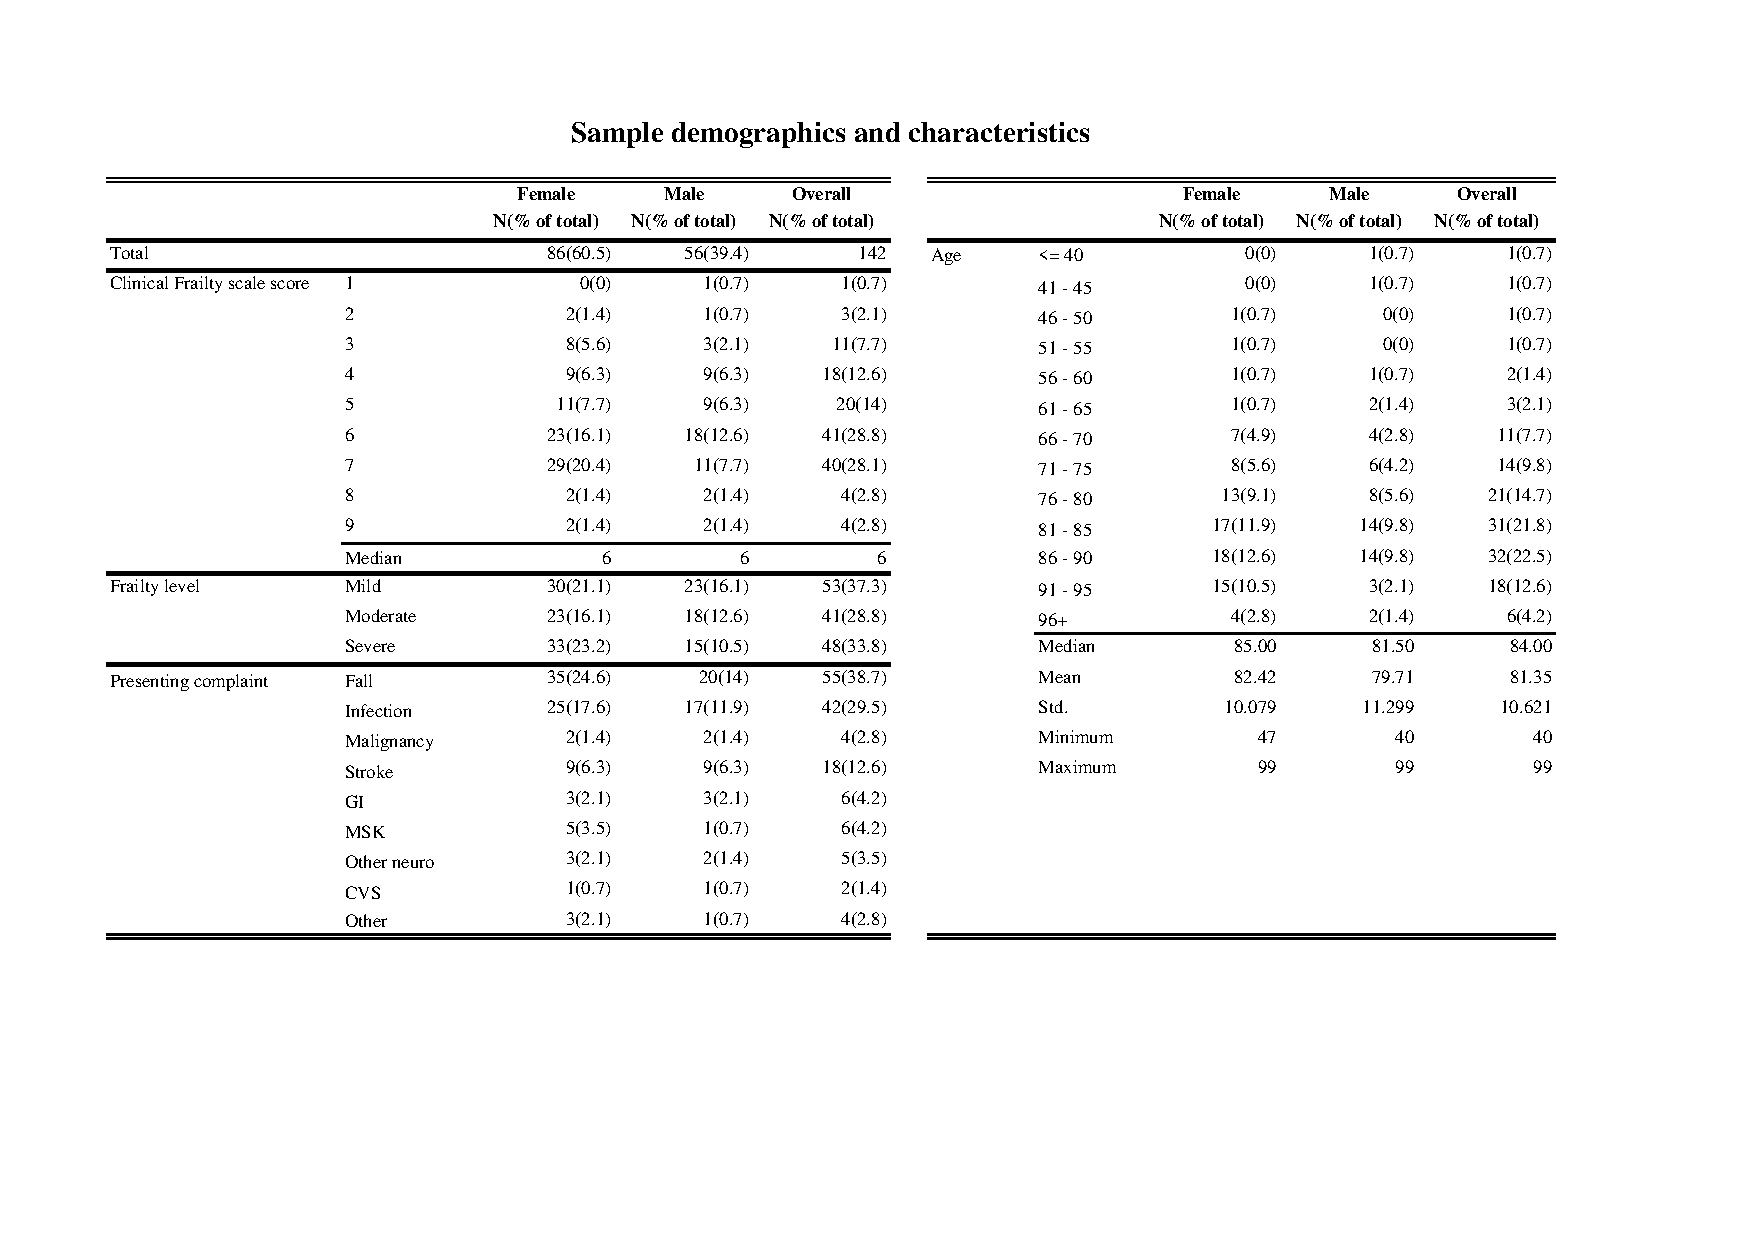
\includegraphics[width=\textwidth,
	trim={1.5cm 4cm 2.5cm 2cm},
	clip,
	angle=90,
	scale=1.45]{media/dist-overall}
\end{table}

Patients in the sample group were relatively old: the mean age of patients was 
81 years with a median of 84 years. The youngest was 40 with the oldest being 
99. Increased age was associated with increased CFS (Spearman's rho
$p=0.016$). 
The initial presenting complaint was not evenly spread. Almost 80\% 
were originally admitted with one of the top three complaints: Fall 37.8\%, 
infection 29.1\% and stroke 12.2\%. 

When viewed by CFS, the distribution shows a high level of frailty. The median 
CFS was 6 - moderately frail, with only 36.5\% of the sample being less frail
than this. Having said that, only just over 8\% of the sample had a CFS of 8
or 9, with 55\% of the sample having CFS of either 6 or 7 - moderate or
severe frailty. This corresponds with the estimation from the literature that 
the prevalence of CH frailty is in the range 24.7\% to 80\%.

When frailty is grouped as described in Section~\ref{ref:cfs-grouping} the 
distribution is much more uniform with mild, moderate and severely frail
representing 36.5\%, 27.7\% and 35.8\% of the sample respectively.
See Figure~\ref{fig:chart-dist-frailty-level}. There was no significant 
difference in level of frailty between the genders ($\chi^2$, $p=0.476$).
\label{sec:results-dist}

\begin{figure}[ht]
\centering
\caption{Distribution by frailty level and existence of ACP on admission}
\label{fig:chart-dist-frailty-level}
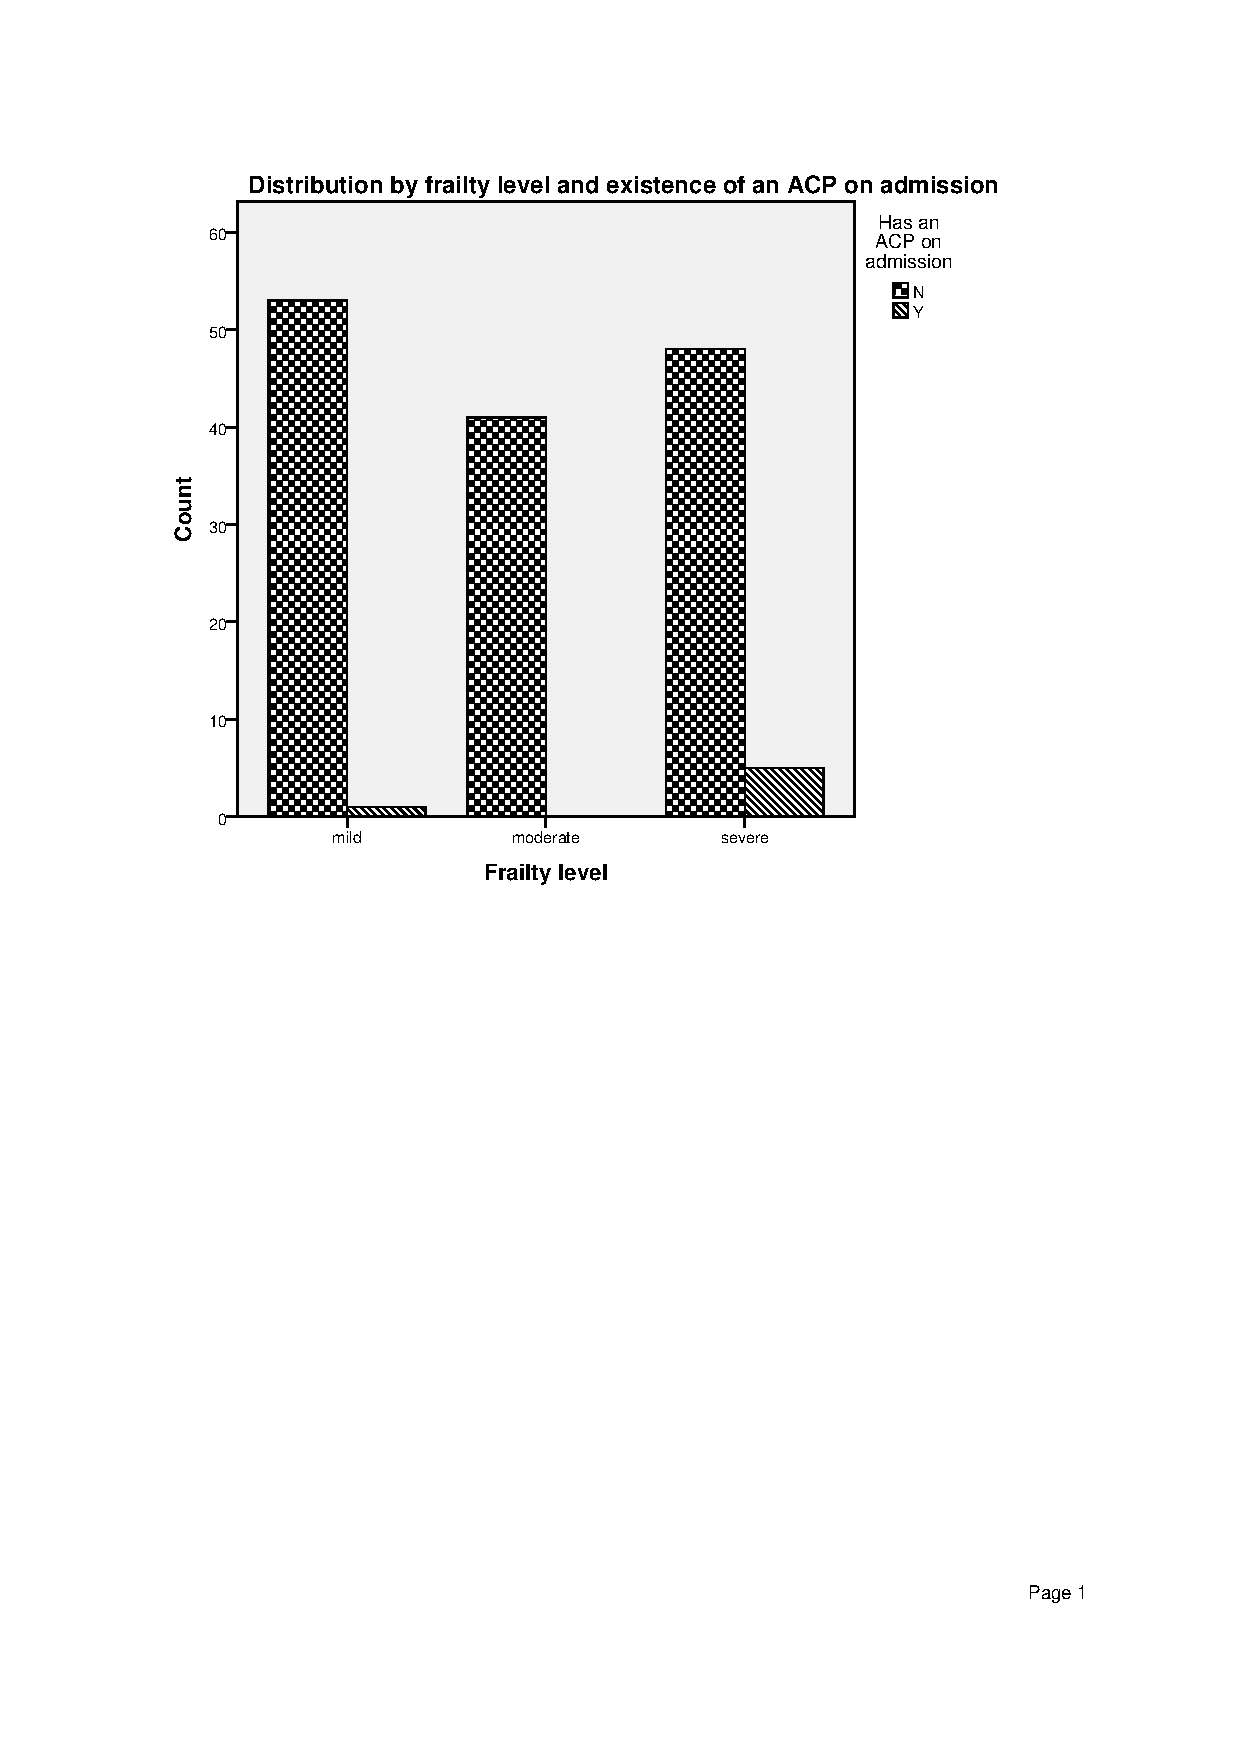
\includegraphics[width=\textwidth,
	trim={2.5cm 14cm 2.5cm 2.5cm},
	clip]{media/chart-dist-frailty-level}
\end{figure}

Very few patients had a preexisting ACP on admission to CH: 6
patients (4.1\%), see Figure~\ref{fig:chart-dist-frailty-level}. There was no 
significant difference in this for the genders (Fisher's exact test, $p=0.223$).

\section{Advance care planning}

The six patients that had a preexisting ACP on admission to CH 
were discounted from future analysis leaving a sample of 142. Of these 18 
(12.7\%) had ACP during the hospital stay. There were no patients that 
declined ACP. The statistics regarding association between the independent 
variables; CFS, frailty level, age, gender and presenting complaint; and the 
dependent variable of whether ACP happens is presented in 
Table~\ref{tab:statistics}.

\begin{table}[ht]
\centering
\caption{Summary of statistical analysis}
\label{tab:statistics}
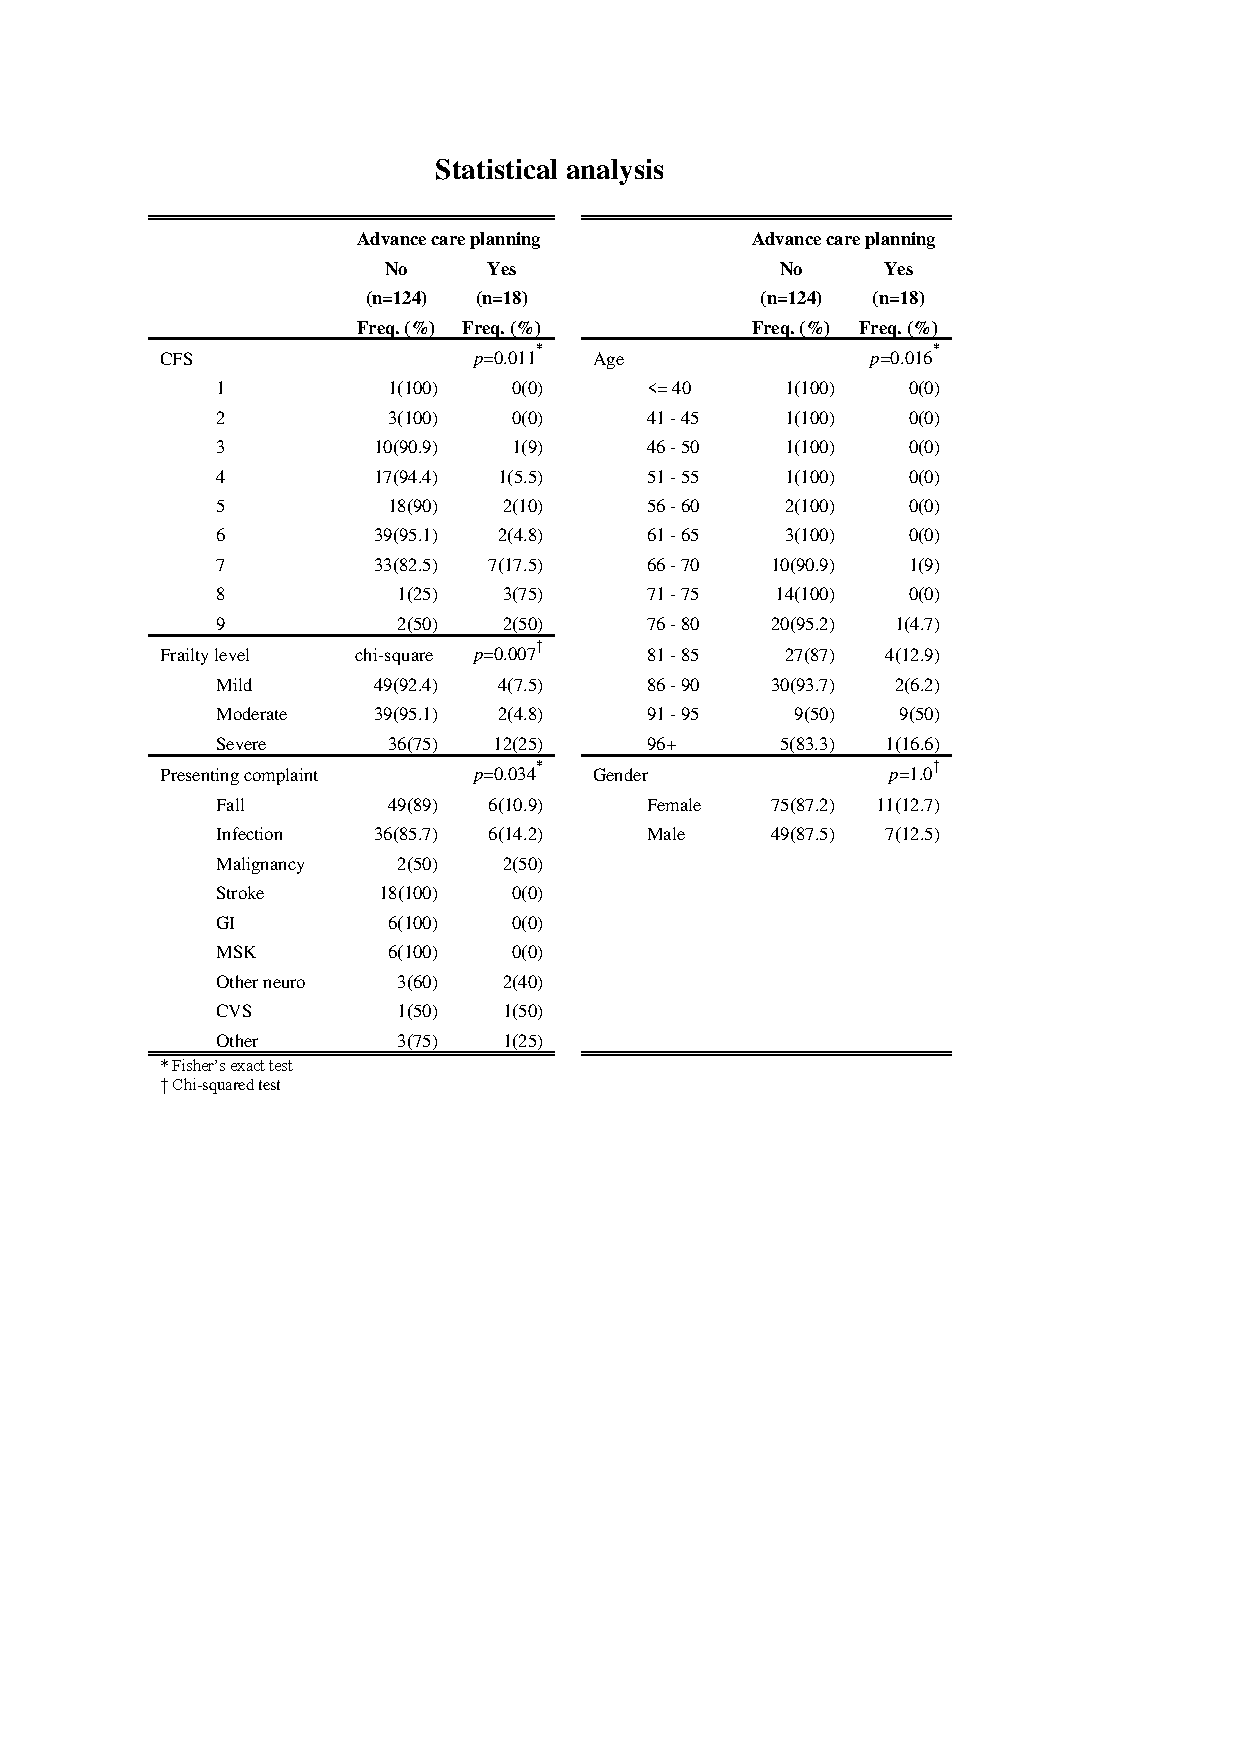
\includegraphics[width=\textwidth,
	trim={2.5cm 10cm 2.5cm 2.5cm},
	clip]{media/statistical-analysis}
\end{table}

\subsection{CFS}

The most common CFS score of patients 
who had ACP during CH stay was CFS=7. Out of the 18 patients that
underwent ACP in the CH, 7 of them (38.9\%) had a CFS of 7. This represents 
17.5\% of the patients with this CFS. The CFS score which had the highest 
proportion of it's patients having ACP was CFS=8 where 3 out of the 4 patients 
with this CFS underwent ACP ($p=0.011$). 


\subsection{Frailty level}

When frailty is grouped into mild, moderate and severe, we saw in 
Section~\ref{sec:results-dist} that the
sample was relatively evenly distributed. 
Whilst about one-third of the sample were severely frail, two-thirds of all 
patients who underwent ACP were in this frailty category. One-quarter of
the patients with severe frailty underwent ACP, compared with mild and moderately
frailty of which 7.5\% and 4.9\% respectively had ACP ($p=0.007$).
Figure~\ref{fig:chart-frailty-level-acp} illustrates this.

\begin{figure}[ht]
\centering
\caption{Advance care planning within frailty levels}
\label{fig:chart-frailty-level-acp}
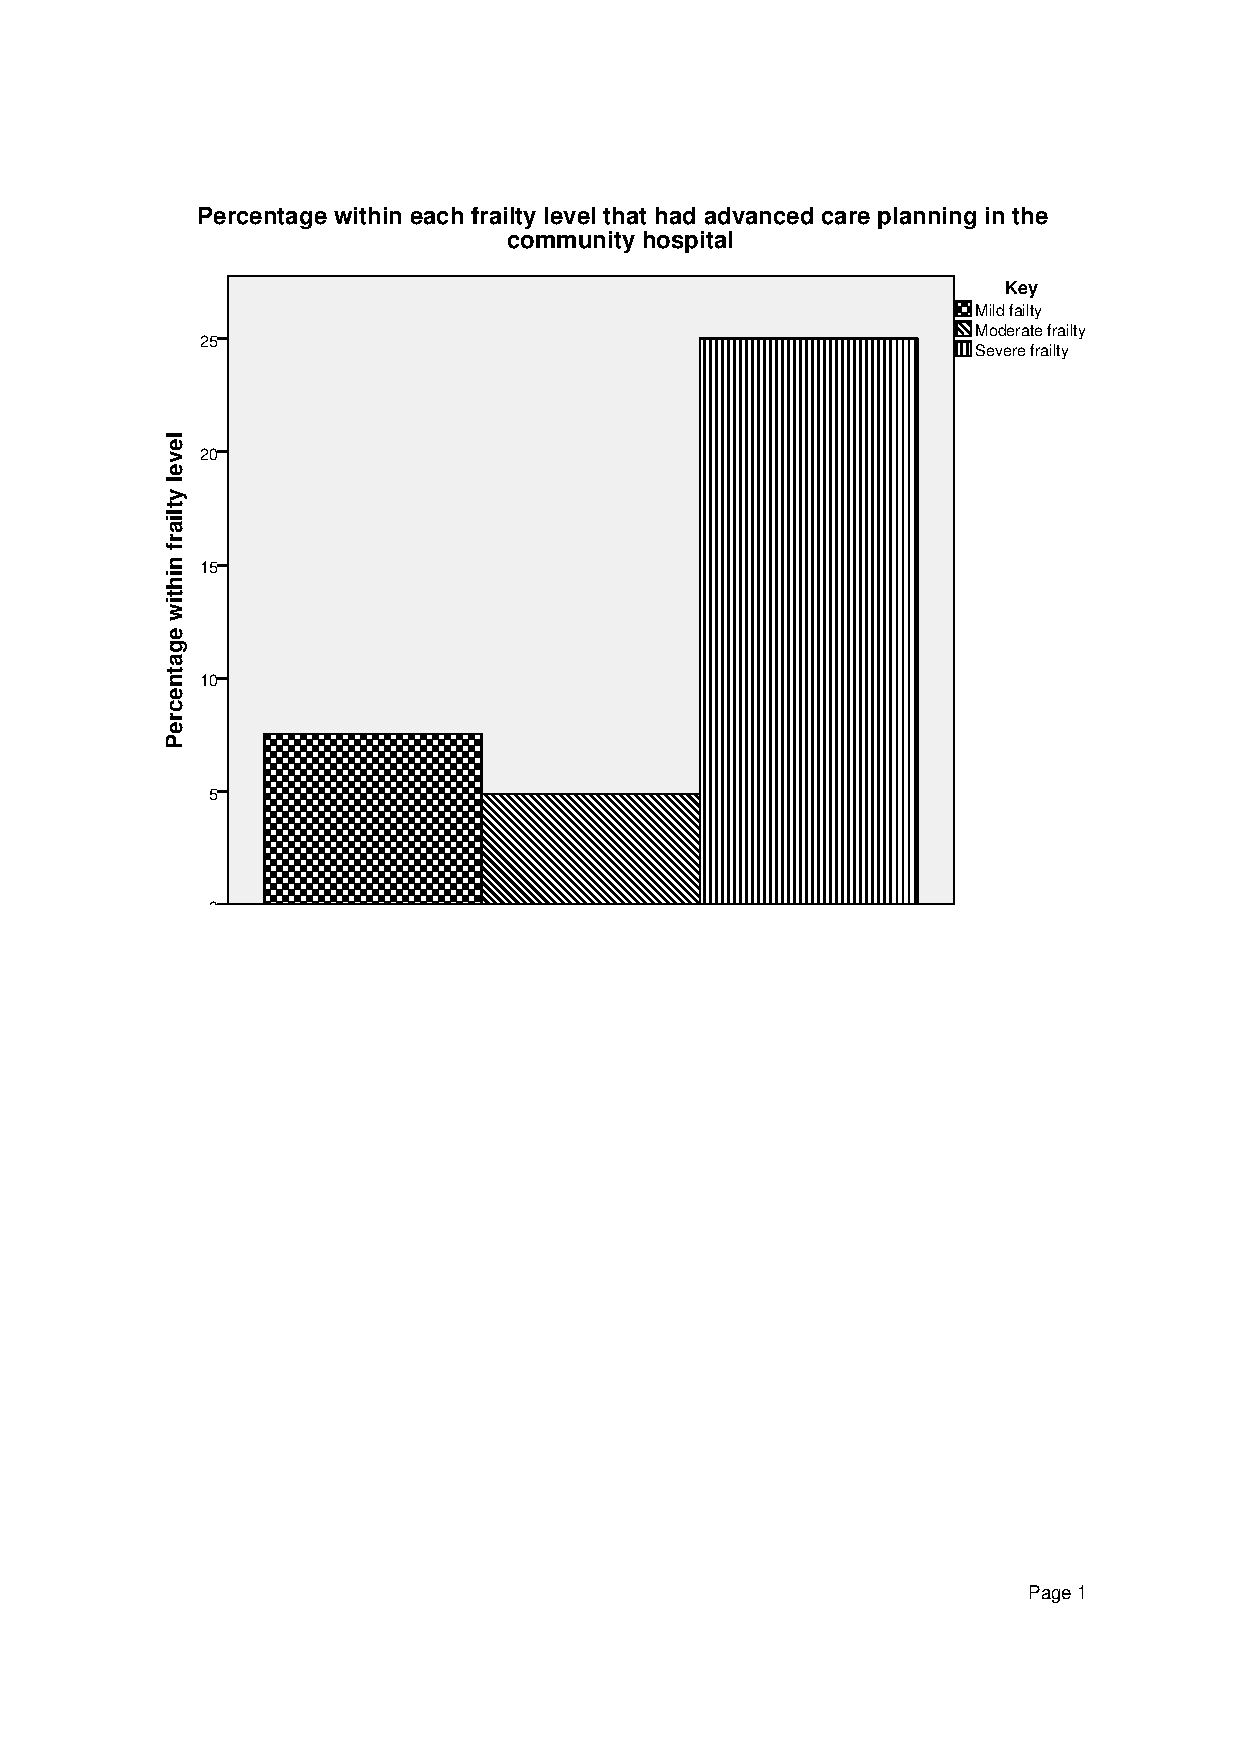
\includegraphics[
	width=\textwidth,
	trim={2.5cm 16cm 2.5cm 2.5cm},
	clip]{media/graph-frailty-level-acp}
\end{figure}

\subsection{Gender}

There was no significant association between gender and ACP: 12.7\% for
females and 12.5\% for males ($p=1.0$).

\subsection{Age}

Age was associated with ACP ($p=0.016$). No-one under the age of 66 
received ACP. Half of the 18 patients aged between 91 and 95 years underwent
ACP but only 6.2\% of those in the 86 to 90 year old category got ACP. This
association is not monotonic and is illustrated in 
Figure~\ref{fig:chart-age-acp}.

\subsection{Presenting complaint}

There was a significant association between presenting complaint and ACP
($p=0.034$). None of the Patients that presented with a primary diagnosis of 
stroke or a GI or MSK disorder 
had ACP. All the other categories had proportions of patients that had ACP
ranging from 10.9\% (fall) to 50\% (both malignancy and CVS).

\begin{figure}[ht]
\centering
\caption{Percentage that got ACP by age group}
\label{fig:chart-age-acp}
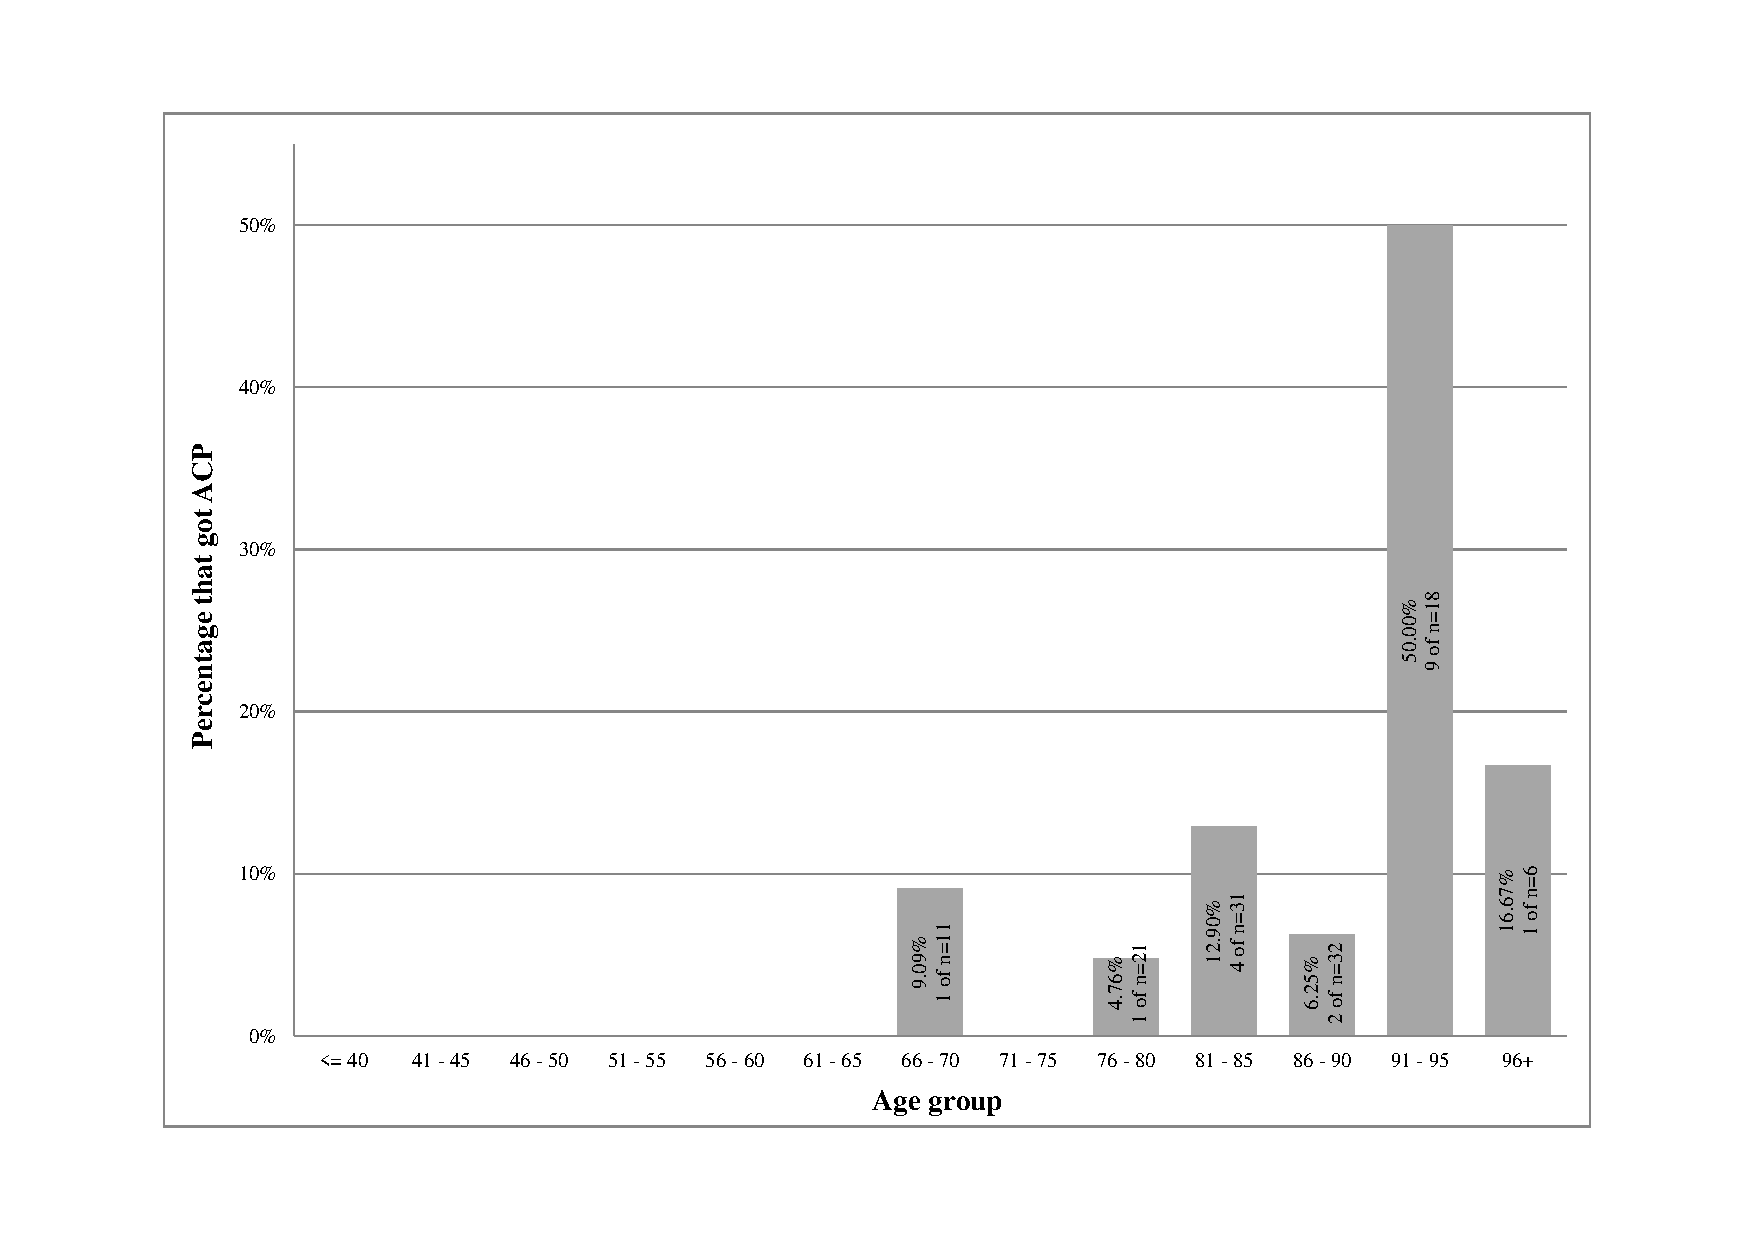
\includegraphics[
	width=\textwidth,
	trim={2.5cm 1.5cm 2.5cm 1.5cm},
	clip]{media/chart-age-acp}
\end{figure}

\section{Limitations to the study}

This study has provided some useful data revealing some interesting findings.
There are aspects of the work that has been done
that could be improved upon. These will now be discussed.

\subsection{Methodology}

Associations have been identified between patient factors and ACP, but
how decisions are actually made has not been explored. To do this would need 
some qualitative work to explore the thoughts of the practitioners involved
in this. Therefore adopting a mixed methods approach 
would maybe have provided richer data, filling in some of the gaps left in the
knowledge that has been generated which would hopefully be more useful still.

\subsection{Sampling}
A non-probabilistic convenience sampling method was employed, which facilitated 
exploration of the subject area. However, the way that the sampling was 
structured meant that some patients, for example those on non-EPR wards, had
zero chance of being in the sample. This questions how representative the sample
was of the CH population, limiting generalisability even at the local level 
\parencite{biggam:15}.

A further issue is presented by the seasonal 
nature of the sample; only patients who were in hospital in the winter were 
included. This could affect the presenting complaints of patients in the sample,
possibly skewing the data.
Conducting the study at a different time of year could have yielded different 
results. A strategy that would have produced results that are more generalisable
to the local system would have been to sample patients from across
a 12 month period. In this particular situation this would have been much more
time consuming because the EPR had been rolled out during the last 12 months in
the Trust, so paper records would have had to be recalled and studied for many
of the patients. 

In defence of the sampling strategy that was used, it has enabled a quick 
snapshot to be generated and the area of local frailty and advance care planning
has been explored, identifying issues that can be
addressed or examined further. The audit could easily be revised or repeated 
over a longer time period. At this juncture all the wards 
will have been on EPR for a substantial period of time so
allowing a probabilistic sampling method to be employed.

\subsection{Reliability} 

Given that this study formed a Master's dissertation there was a limit to the
amount of time in which the project had to be undertaken. To speed up data 
collection, help was given to the author by a few
colleagues, who each accessed small subsets of the sample patient records to 
extract data. Much of the data is unambiguous: age, gender, presenting complaint
and whether ACP happened. To ascertain the CFS it is necessary to interpret 
information about the patient from the records to decide the score. The
inter-rater reliability of the CFS has been questioned \parencite{gilbert:18},
so it is possible that, 
if the study were to be repeated, the results may not be identical.
To defend the use of the CFS in this context, it is quick to calculate, usually 
less than 1 minute \parencite{elliott:17}, and it is used in the local acute
Trust and so in the future would facilitate comparisons of serial frailty
scores.

\subsection{Bias} 
During the period of data collection, the author was working outside the Trust 
so was not involved in the care of any of the patients sampled. This hopefully 
allowed objective interpretation of the notes and associated decision making.
The colleagues who assisted with some of the data collection were working 
within the Trust at the time, but measures were taken to reduce the risk of 
bias. They were allocated patient notes from wards where they had not been
working and there were instructed to contact the author if they discovered
anything which made them question the quality of clinical practice. No such
findings were reported.

\subsection{Results and findings}

The study was limited to 8 of the 12 wards in the Trust. Two of these wards
are stroke wards and the four wards that were not included in the study were 
general wards. Therefore the proportion of patients in the sample
who were admitted following stroke is likely to have been higher than if the 
study was to be repeated taking a sample from across all the wards. There may 
well be different attitudes towards advance care planning for patients whose
primary reason for admission was stroke when compared to the patients who
were admitted for another reason.

Stroke is potentially very life changing. Stroke can happen at any age with 
around a quarter happening in people of working age \parencite{stroke:18}. 
Therefore, people undergoing 
inpatient stroke rehabilitation have a wide variety of premorbid functional 
abilities and thus varied premorbid frailty. These variations will
affect the feelings of the patient and their attitudes to future care and will
likely influence the decision making around ACP that the team make. Another
possible factor is that the consultants with responsibility for the stroke 
patients are specialist stroke physicians and will have slightly different 
thought processes to the geriatricians who work on the remaining wards.
and treatment.

\chapter{Discussion}

\section{Community hospital frailty}

The first part of objective~\ref{obj:prevalence} is to assess how frail the
local community hospital population is. It was seen in 
Section~\ref{sec:local-practice} that the primary reason that many patients are
admitted to community hospital is for rehabilitation. A number of implications 
can be 
drawn from this. Firstly that they have a level of dependence on others for 
activities 
of living and secondly that healthcare professionals feel that there is 
potential for this dependence to be reduced through a period of rehabilitation. A 
third implication is that this therapy cannot be undertaken in the home
environment due to the current high level of dependence.

The validated CFS that has been employed in this study uses the position of a person
on the continuum of independence and dependence to grade their frailty. It
would be expected, therefore that people undergoing such inpatient rehabilitation 
would score relatively highly on the CFS, and thus the frailty level of the 
CH population would be high. The results of this study bear this out in that
almost two-thirds of the sample were either moderately or severely frail
and the median CFS was the moderately frail score of 6. There was minimal
difference in the level of frailty between the genders.

The sample is considerably more frail than the general population. 
\textcite{collard:12} performed a systematic review to assess frailty in older
people, and found that, in the over 85s, the prevalence of frailty is about
26\%. \textcite{clegg:13} agree with this noting that the prevalence of frailty
increases with age. Over one-third of the sample were severely frail. This could
be expected because having frailty makes a person more prone to needing to be
admitted to hospital. People of the same age who are resilient against
minor stressor events do not need hospital admission, so the population of older
people in hospital is likely to be frailer than the general population.

\section{Preexistence of advance care plan}

Just over 4\% of the sample had a preexisting ACP on admission to CH. 
\textcite{clarke:14} judged that at least 28\% of acute hospital 
inpatients are in the last year of their life, suggesting that advance care 
planning should be considered for these people. 
These two numbers are very different, however the majority of CH patients 
come directly from an acute hospital
stay, so it could be argued that we would expect about 28\% of them to be in
the last year of life. However, it is clear that patients who are transferred 
from acute hospital to CH are a specific subset of those admitted acutely.
This subset obviously does not include those that die whilst in an acute bed,
all of whom would contribute to the 28\%.  However, the CH subset is likely 
to be generally more frail than the acute hospital population; whilst some
acute patients are too frail to benefit from CH admission, there are also many 
who do not need rehabilitation and thus avoid CH.

On balance, it is likely that the proportion of CH inpatients that are in the
last year of life is roughly similar to this acute hospital figure. It
could be argued that, if you are likely to die within a year, healthcare
professionals involved in your care should be helping you consider what
is important to you for the future and planning for this. 


GPs in England are contractually required to identify those patients who are 
over 65 years old and have severe frailty and to review them clinically
\parencite{nhse:17}. There is a financial incentive if they then
engage in ACP with the patient \parencite{hunt:16}. Given
this, it would be expected that more than 4\% of CH patients arrive there
with an ACP already in place. Perhaps the community hospital has a role in
ensuring that one is in place by the time they leave the hospital.

\section{Associations with advance care planning}

In this study both age and frailty were associated with increased incidence of
advance care planning. There was also a weaker but still significant association
between presenting complaint and ACP. Formal frailty assessment is not 
considered in the CH when practitioners think about whether or not ACP is 
appropriate for that patient at that point in time. Such decisions are normally
based on subjective judgements which take into account many factors related to
the patient.

We saw back in 
Section~\ref{sec:frailty-implications} that, while frailty is not an
inevitable consequence of getting older, it's incidence does increase with age,
and increased age was associated with increased frailty in this study. It seems
that there is a three way association between age, frailty and advance care 
planning, and as such it is not possible to tell whether either factor of 
age or frailty influences ACP. 

The other factor that had an association with ACP was presenting complaint.
Falls and infections accounted for the presenting complaint of two-thirds
of the patients who received ACP. These were not the presenting complaints
with the highest percentage of their patients getting ACP; malignancy, other
neurological, CVS and other all scored higher on this, but their overall numbers
were very small. Out of these, other neurological was the highest with 5 patients in 
total, 2 of which got ACP. These numbers are so small that the significance
of their higher proportions of advance care planning is questionable. 

\subsection{Falls}

The \textcite{bgs:14} describe five `frailty syndromes' as presentations or 
symptoms that are actually sequelae to an underlying pathological process
that has manifested itself in this way because the person has frailty
(see Appendix~\ref{apx:syndromes}).
Someone presenting with one of these raises the suspicion that they have frailty,
and therefore they should be screened for frailty at this point.

Falls are one such frailty syndrome and were the most common reason that someone
in this study was originally admitted to hospital. It is possible that these
people were, on average more frail and that was the reason that a 
relatively high proportion of people admitted with falls got ACP.
This study did not examine the other four frailty syndromes. 
It would be interesting to assess whether there is 
any association between the incidence of the individual frailty syndromes 
in the sample and both frailty and advance care planning. Here we have only
examined a link between one of the frailty syndromes and ACP and this
provides an incomplete picture.  

\subsection{Infection}

A defining consequence of living with frailty is that when a person 
experiences a relatively minor stressor or insult, such as an acute infection, 
they are at a greater risk of adverse outcomes. Their physiological reserves
are reduced to the extent that they are living just above the thresholds 
for adverse outcomes to occur. This means that when they get an infection
they are at a much higher risk of needing admission to hospital. This explains
the frailty syndromes: the frail person who gets an infection is at a high 
risk of developing one of these syndromes, each of which increases their 
dependence on others.

This combination of acute infection and increased dependence can be a trigger
for acute hospital admission. They are then treated for the acute problem,
infection, and when they become medically stable they no longer need an acute
bed. The frailty syndrome may well persist after this, leading to the
need for a period of rehabilitation, hence community hospital admission.

The story so far suggests that many patients who are originally admitted 
due to infection and 
subsequently arrive at a community hospital are severely frail individuals.
A relatively high proportion (14\%) of such patients in this study received
advance care planning. The clinical team looking after them realised that they
would benefit from ACP. The data does not tell us what the factors were that 
influenced this reasoning. The fact that they were admitted with an infection
is an unlikely influential factor because 85\% of such patients did not get
ACP. It could be argued that they the real reason for their initial admission
was their underlying frailty with an infection triggering on of the frailty 
syndromes. If this is the case then it is likely that frailty is more likely 
to have been an influential factor for ACP than their infection was. Again, 
investigating deeper into frailty syndromes and ACP should help to clarify 
this.

\section{Influential factors}

Whilst the age of the patient
had an association with the advance care planning ($p=0.016$), as did 
presenting complaint ($p=0.034$),
the common factor here is frailty. Level of frailty had the most 
significant association, $p=0.007$. Increased age makes it more likely for a 
person to be frail, so the age association could be partly due to frailty
increasing with age. We have seen above how the presenting complaints of 
falls and infection are possibly manifestations of the frailty of the patient.

Objective~\ref{obj:association} talks about identifying which factors 
influence advance care planning.
The theme of frailty as the main candidate influencing factor runs through.
For a factor to influence whether something happens or not implies that there 
is a cause and effect relationship between the factor and the outcome. 
The effect has occurred in the thought processes of the clinical team. To 
explore these thought processes would provide an insight into how decisions
have been made, an undertaking which is beyond the timescale of this study.

Associations have suggested influencing factors, and further reasoning based
on knowledge of frailty has enabled a suggestion to be formed that frailty
does influence advance care planning. However it could equally be argued
that age influences ACP. There is no evidence in this study that patient
gender influences ACP. The situation surrounding presenting complaint as
an influencing factor is unclear.

In this patient cohort there is great complexity, due in part to frailty
of the patients. The presenting complaint is indeed a factor that has 
necessitated a hospital admission, but there are often other underlying
factors contributing. There is an association between presenting complaint
and ACP. Due to the complexity of the patients there are likely to be many
interacting factors. These will interact with each other and understanding
the influential role of each is not trivial.
It might be that, in patients with
frailty, the presenting complaint has less influence on their care journey than
it would have for people without frailty who are admitted with a similar
complaint, due to the complexity provided by the additional factors that
come with frailty.

\section{Recommendations for practice}

Community hospitals should be identifying patients that are moving toward the
end of life and offering them advance care planning \parencite{dh:09}.
When the OOH service review a patient they often do not know them. It is 
suggested by \textcite{brettell:18} that if the in-hours team can provide more
complete information about patient circumstances as they are approaching the
end of life then the OOH service can make decisions that are more appropriate
to the situation. To achieve this, the community hospital day team need to be 
better at recognising that a patient is nearing the end of life, and then 
using this knowledge to engage with the patient and their relatives and 
carers to ascertain what is important to them. This can then be used to 
produce an ACP that the OOH practitioner can use to inform their decision
making. Severe frailty is a factor that should be used to trigger consideration
that a patient may be entering an end of life phase, thus initiating this
communication process.

The sample population was relatively frail. Frailty puts a person at an 
increased risk of adverse outcomes, including death, and a significant
proportion of the sample are likely to have been in the last year of their life.
These people deserve dignity at this stage of life and they are likely
to appreciate being involved in making decisions about how their health is
managed at this point and looking forward. Only a very small number of these 
people had been engaged in such processes prior to them arriving in the CH.
Whilst there, only 13\% of them benefited from an ACP process. A small 
proportion when compared to the 35.8\% that were severely frail.

Frailty 
appears to be the biggest factor likely to be influencing ACP, but we are 
clearly
not offering ACP to all those who are severely frail. It seems therefore that
the level of frailty of CH patients should be formally assessed. If they 
are found 
to be severely frail, this should trigger us to consider whether advance 
care planning should be offered to that person whilst they are an inpatient.

The CFS is easy and quick to use \parencite{elliott:17}, and it is used in the 
local acute Trust. 
Using the CFS in the CH would allow for comparisons to be made between the CFS 
as calculated on initial admission and then later in their inpatient journey
when more is known about them. If the second frailty score is higher than the
first this could signify advancing frailty despite medical management, 
and would question the value of future medical treatments for this person.
In such instances advance care planning needs to be considered. 

In summary, frailty should be assessed in community hospitals. The frailty score
that should be used is the CFS. When this is done the score should be compared
with any previous CFS for the patient. If the CFS now is greater than previous
or is greater than 6 then advance care planning should be considered.

\section{Recommendations for future research}

This study has provided an insight into the amount of frailty in the local
community hospitals and has also given an idea of what factors influence the 
decisions that are made around advance care planning. It has been possible to
draw on these findings and recommend how practice should change to benefit
patients locally. However, there have been a number of questions that have 
arisen throughout the process, leading to a desire for formal research to 
search for some answers. 

It has emerged that the patients involved are complex and that making decisions
about their care is complex also. There has been suggestions that frailty is 
a major factor in deciding whether a patient should have ACP. This is not
clear, nor is the role played by other patient factors. To gain more 
understanding of this some qualitative research is needed 
to explore the thoughts and feelings of practitioners involved in ACP in
community hospitals. This would hopefully help untangle some of the complexity
that has been discussed.

We have seen that this study has not given us generalisable findings. This
could be addressed by designing a study with a wider setting, including
multiple community hospital Trusts, and a more robust sampling strategy. 
Such a project should
also look at all five frailty syndromes, not just falls. This would help
provide a fuller picture of what factors influence advance care planning.

Discussion has alluded to there being links between age, presenting 
complaint and frailty. This needs to be explored in more detail to
ascertain what associations there are between these variables in CH patients.
This may provide additional clues to the frailty of patients and hence
provide other triggers for ACP.

\chapter{Conclusion}

This chapter will review the initial research objectives and the findings
provided by this study in relation to these. 
Recommendations for practice and future research have been made and these 
will be summarised.
The author
has developed through the process of producing this dissertation so a section
of self reflection will conclude the chapter.

\section{Research objective \ref{obj:prevalence}: Level of frailty in
	community hospitals}

The results showed that the sample was much more frail than the general
population, even when taking age into account. It was suggested that the level
of frailty may actually have been a large contributory factor in patients
being admitted to the CH in the first place, accounting for this difference.
The literature review suggested that the level of CH frailty was in the range 
24.7\% to 80\%. This study found that 63\% of the patients had moderate or
severe frailty, which is congruent with the findings in the literature. Whilst
frailty is common, only 4.1\% of the sample had an ACP on admission to CH, a
surprisingly small proportion.

\section{Research objective \ref{obj:association}: Factors that influence
advance care planning}

Statistical associations were found that suggested that age, presenting
complaint and frailty may all influence ACP. Further discussion elucidated
this, arguing that whilst there are associations, the actual decision
making process needs further exploration to provide clarity. In the absence of
this it has been suggested that the associations with ACP of age and 
presenting complaint may actually be attributable to frailty, strengthening
the argument for further research.

\section{Research objective \ref{obj:recommend}: Recommendations for practice}

Local community hospital inpatients need to be assessed for frailty. CFS is 
the tool that should be used for this assessment. If they are
found to be severely frail (CFS of 7 or above) or their frailty is getting
worse, then advance care planning
should be considered for them.

\section{Recommendations for future research}

Research is required to explore the decision making around ACP in CH. The
link between frailty syndromes and ACP in CH patients needs to be examined, 
as does the associations between age, frailty and presenting complaint.
Future research should be more rigorous to improve it's generalisability
both locally and the wider community.

\section{Self reflection}

This dissertation started slowly. The author knew a few months prior to 
commencement that he wanted to explore the issue of frailty in the community
hospitals, and whether there were benefits to scoring patients for frailty.
Another strand that helped make the link to the chosen route was a feeling
that the author had that too many patients got transferred from CH to acute
hospital when this was not likely to give them the best outcome.

The next stage was when delays happened. The author discussed his ideas with
a number of different colleagues and everyone gave him different ideas about 
what to do. This caused him great confusion, and he struggled to get a single 
plan in his head. In retrospect, these discussions should have been had 
much earlier in the process; ideally before the formal work had started. That
way he would have been able to focus much sooner.

As it was, this confusion in his mind took a long time for him to sort out.
When he eventually did get a definite plan, he then had to work hard to get
the university ethics application submitted in a reasonable time. He was 
encouraged by his supervisor to set a target ethics committee, and this helped
him focus and submit on time. 

Another mistake was made following this. Once the ethics application was
submitted he knew that he would have to wait about 4 weeks until he had
authority from the committee to collect data. He had planned to use this time 
to write the bulk of the introduction and literature review chapters. However
this did not happen. Instead he took too much time off at this stage and
achieved very little during this time period. 

Once ethics approval had been gained he started the data gathering straight
away. He acknowledged that time was running out, and talking to a colleague 
about this, she suggested that he ask people to help collect data. He took
this advice on board and about five colleagues assisted with this, which
helped a lot.

Analysing the data was the next hurdle. Despite being a Mathematics graduate
the author soon realised that his knowledge of statistics was poor. He got 
quite flustered with this for a while before realising that he couldn't just
dip into his SPSS statistics book at various points and hope to understand
what he was reading. He went back to the start and read the basic stuff first,
then finding that the material about the actual tests that were appropriate to
this project made sense. The learning point here was not to try to take 
shortcuts with learning about things you don't understand.

There have been many times when the author has found himself staring at the 
computer screen, having no clue how to proceed with writing. He has got quite
frustrated at times. Taking time out when this happened was what he learnt to
be useful. It took the frustration away, allowing him to eventually organise
his thoughts whilst away from the dissertation. This meant that when he next 
sat down to work he was actually productive.

Overall, going through this process has had many benefits for the author. He 
has learnt more about frailty and about how his practice manages it,
specifically in relation to advance care planning. He has also gained a 
better understanding of how he learns best and about how to be more productive.
Most of all he is hopeful that the 
findings that he has made can be used to implement changes to practice that 
will benefit some of the more frail patients that his team encounter.

\printbibliography[heading=bibintoc]

\clearpage

\appendix

\chapter{Clinical Frailty Scale}
\label{apx:cfs}
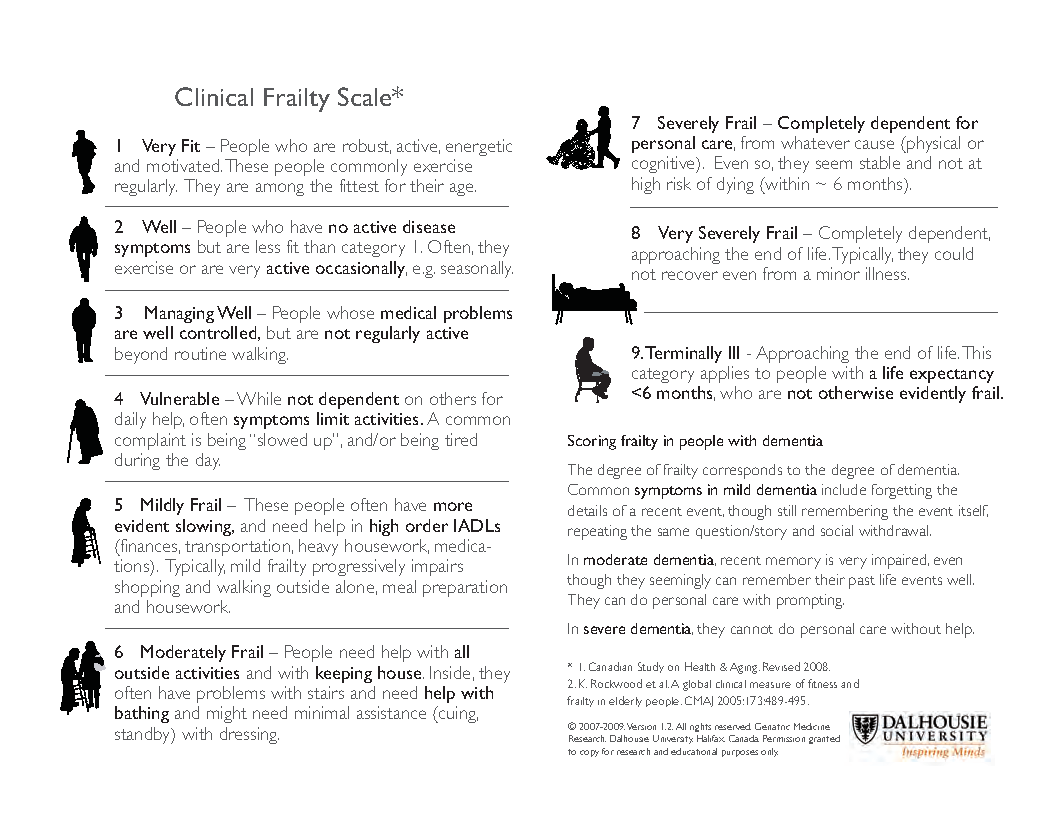
\includegraphics[width=\textwidth]{CFS}

\chapter{Frailty Syndromes}
	\label{apx:syndromes}
	\begin{enumerate}
	\item Falls (e.g. collapse, legs gave way, ‘found lying on floor’).
	\item Immobility (e.g. sudden change in mobility, ‘gone off legs’ ‘stuck in toilet’).
	\item Delirium (e.g. acute confusion, ’muddledness’,
		sudden worsening of confusion in someone with
		previous dementia or known memory loss).
	\item Incontinence (e.g. change in continence –
		new onset or worsening of urine or faecal
		incontinence).
	\item Susceptibility to side effects of medication
		(e.g. confusion with codeine, hypotension with
		antidepressants).
	\end{enumerate}

	\parencite[page 8]{bgs:14}
\chapter{Data collection tool}
\label{apx:tool}
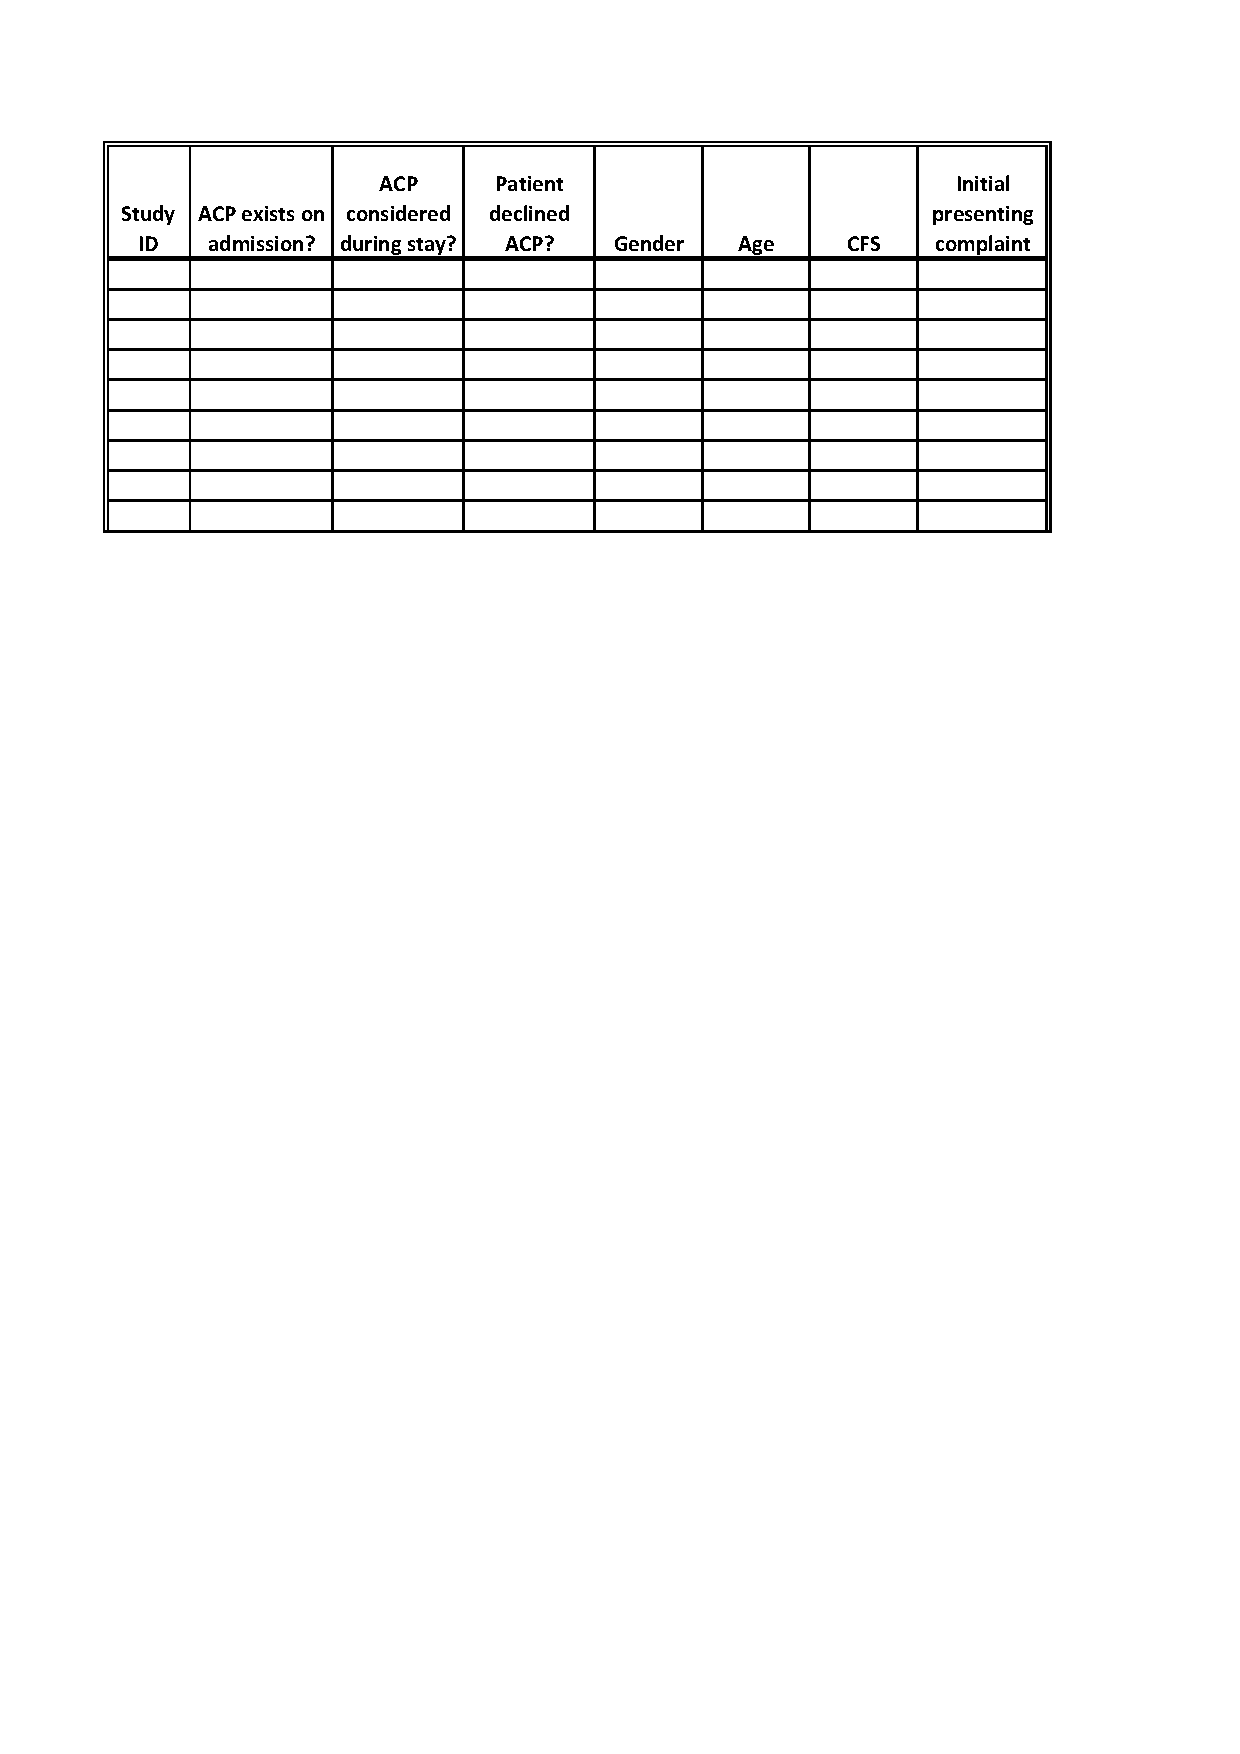
\includegraphics[width=\textwidth,
	trim={0.5cm 13cm 2.5cm 1.5cm},
	clip]{dataCollection}
\chapter{Age distribution analysis}

\label{apx:dist-analysis}

\begin{figure}[ht]
%\centering
%\begin{minipage}{0.45\textwidth}
\centering
\caption{Age histogram with normal distribution curve}
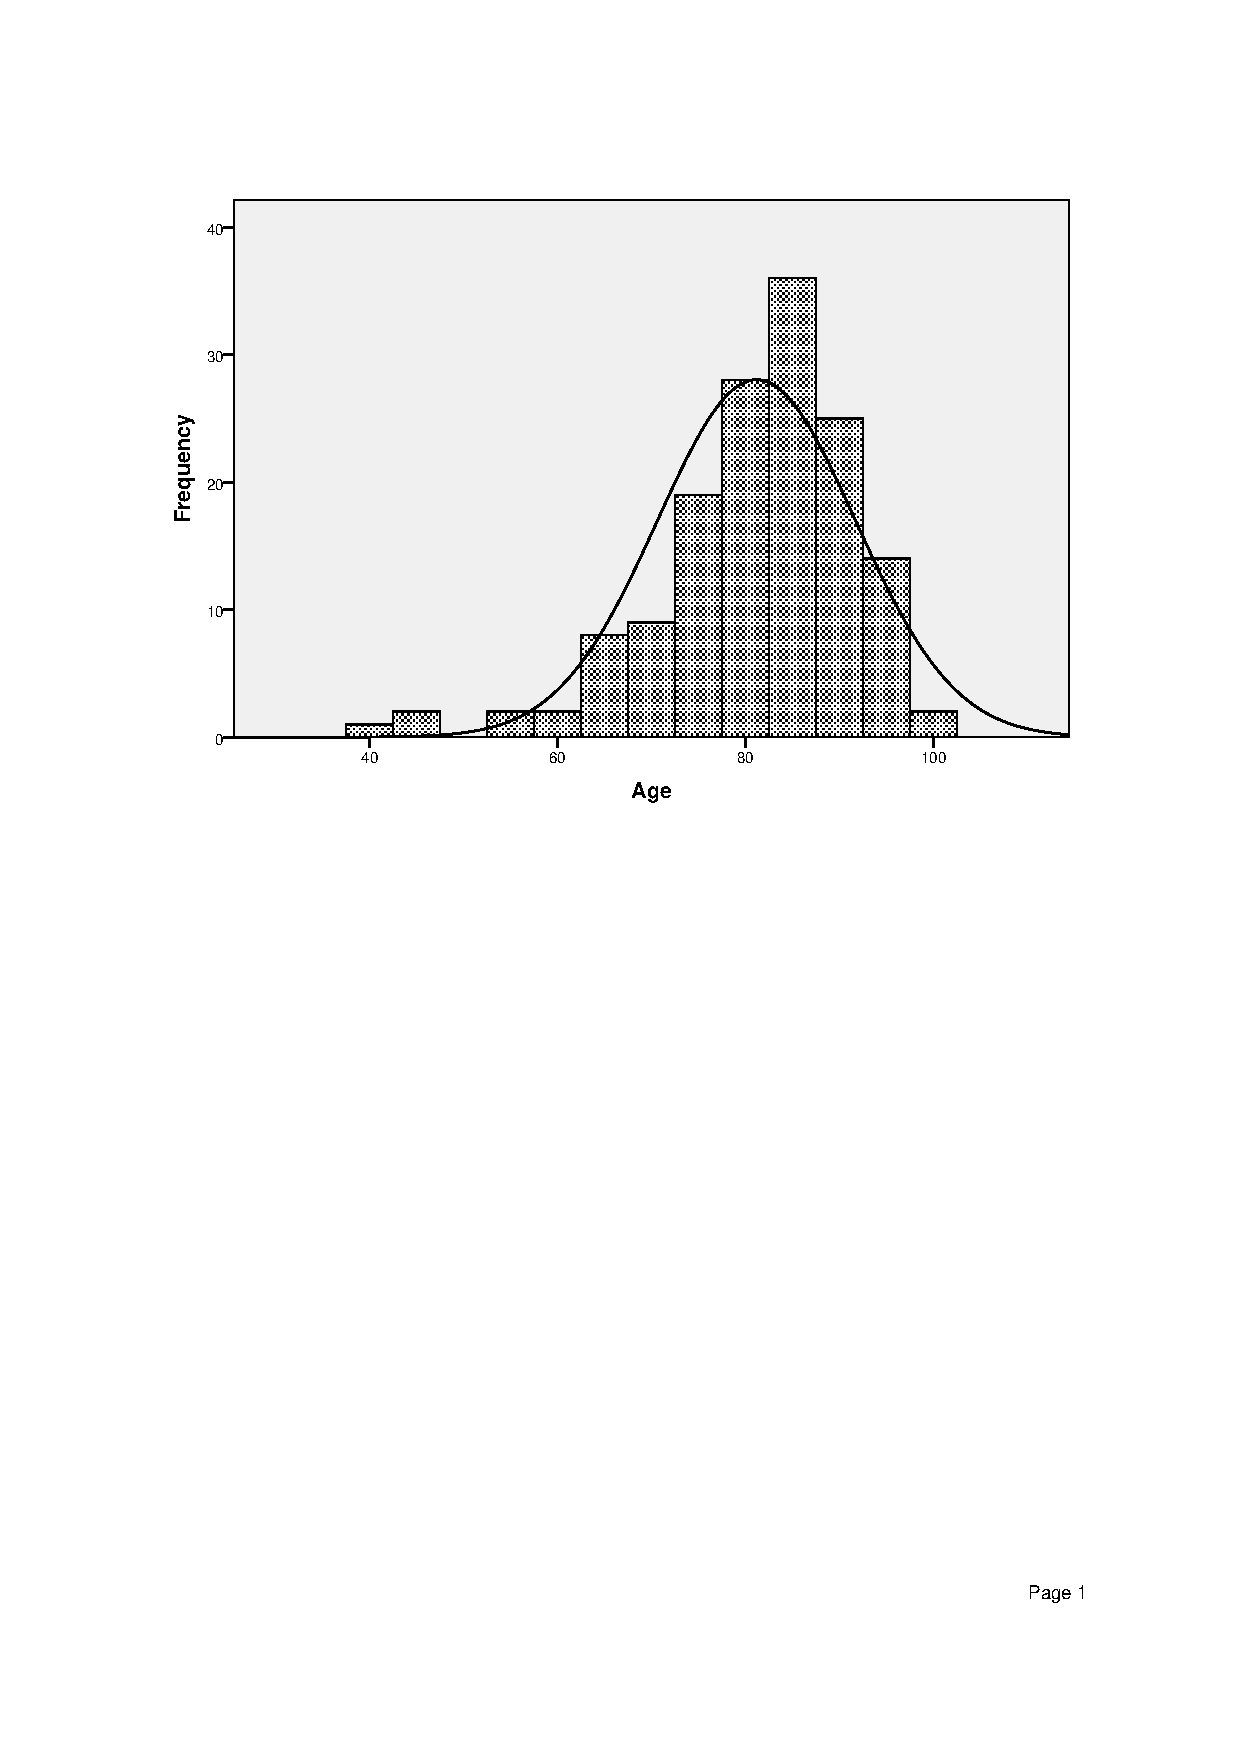
\includegraphics[width=\textwidth,
	%height=\graphdiv\textheight,
	trim={2.5cm 15.5cm 2.5cm 3cm},
	clip]{media/age-normal-curve}
%\end{minipage}\hfill
\end{figure}

%\begin{minipage}{0.45\textwidth}
\begin{table}[ht]
\centering
\caption{Age skewness and kurtosis measures}
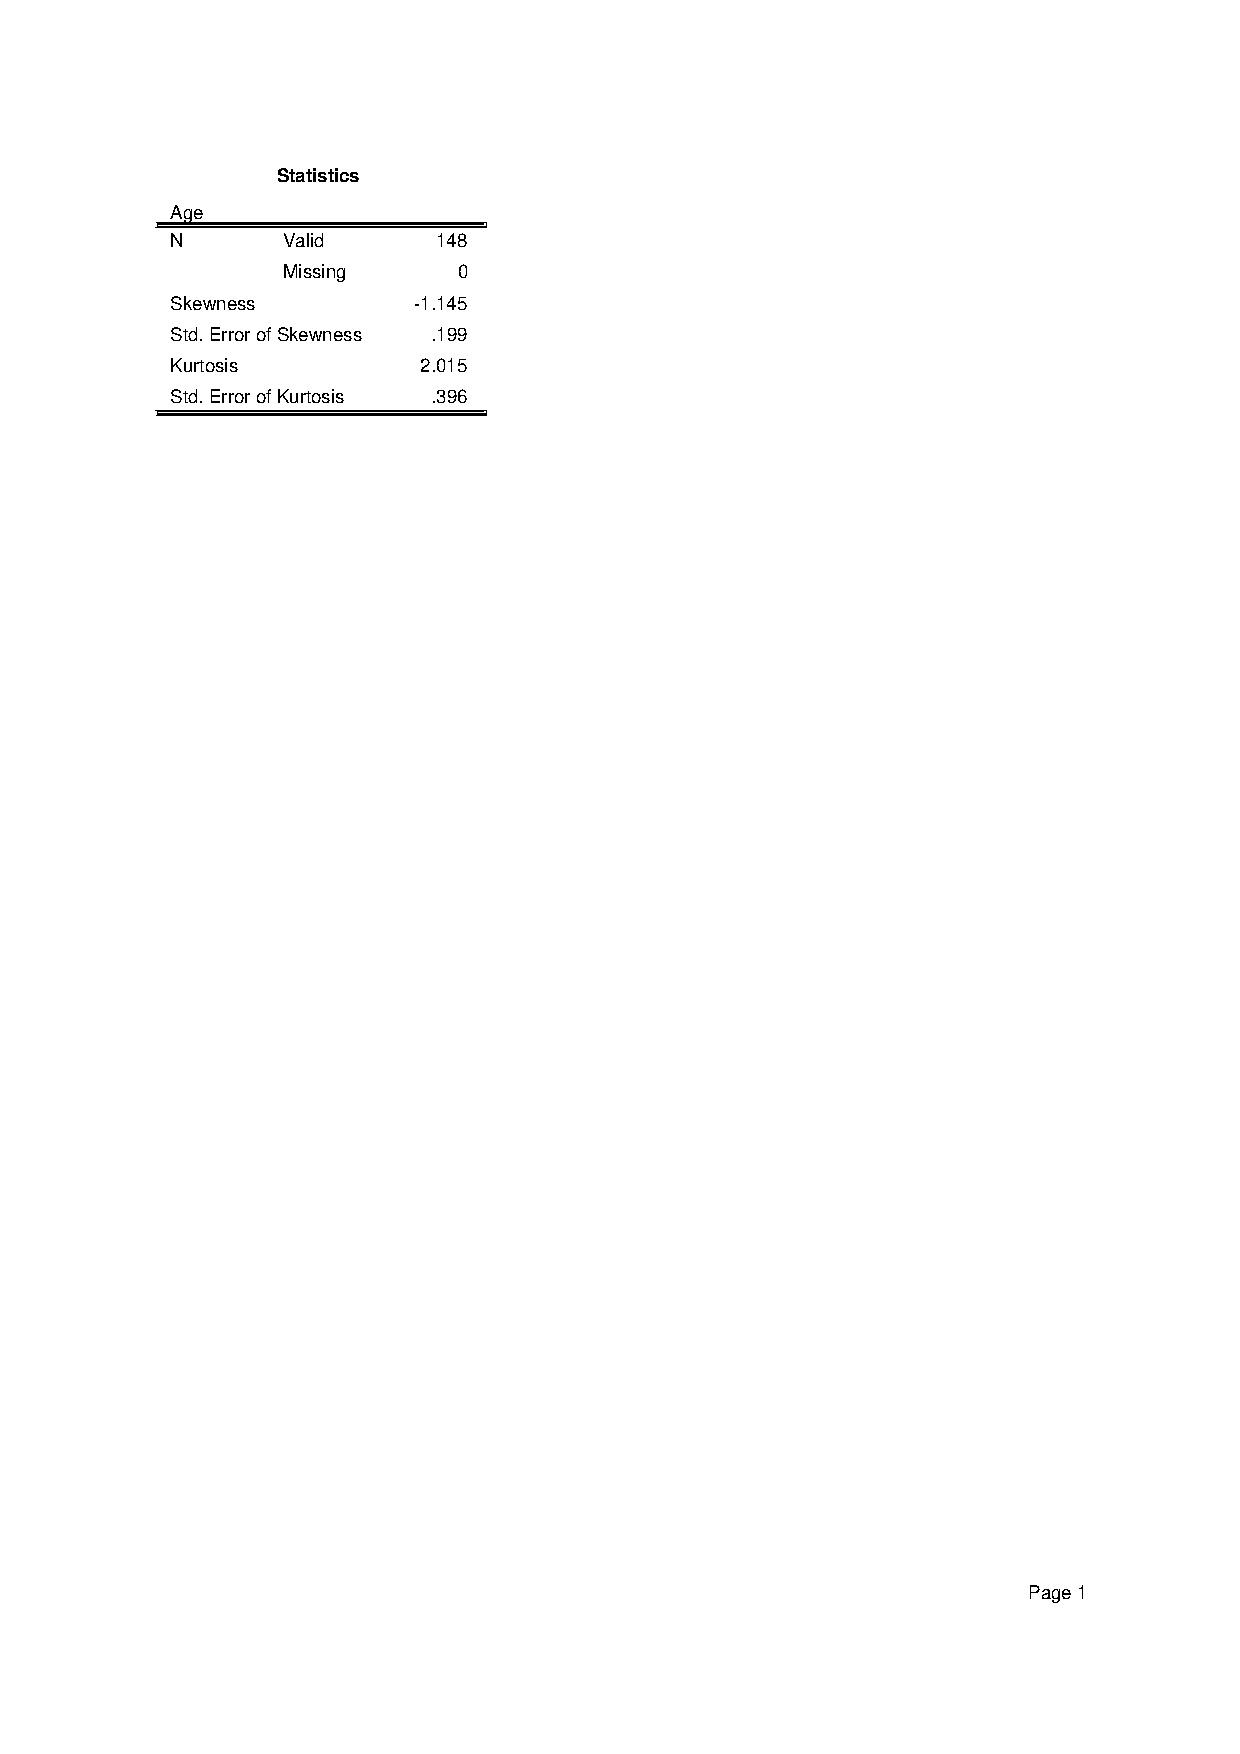
\includegraphics[width=\textwidth,
	%height=\graphdiv\textheight,
	trim={2.5cm 22cm 12cm 2cm},
	clip]{media/age-skew-kurtosis}
%\end{minipage}
\end{table}

\begin{figure}[ht]
%\centering
%\begin{minipage}{0.45\textwidth}
\centering
\caption{P-P plot for age}
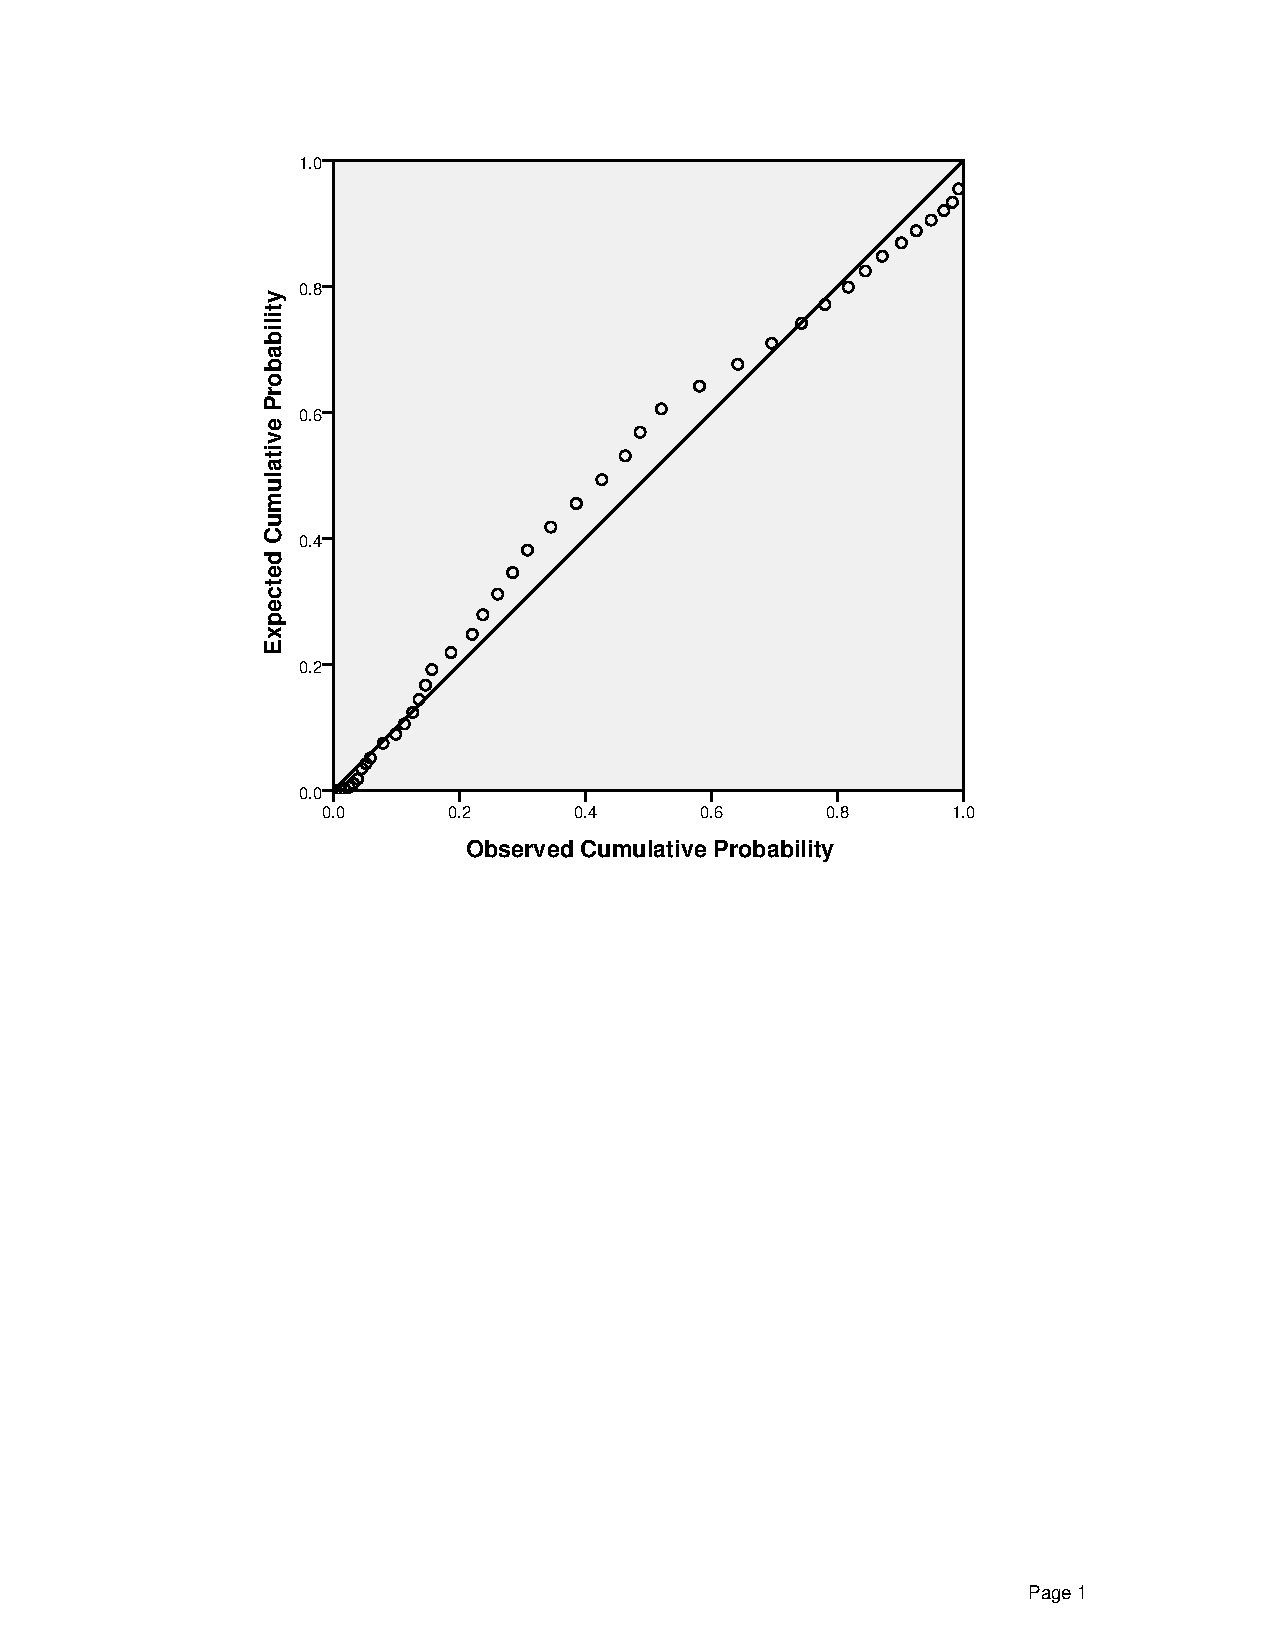
\includegraphics[width=\textwidth,
	%height=\graphdiv\textheight,
	trim={2.5cm 13cm 2.5cm 2cm},
	clip]{media/age-p-p}
%\end{minipage}\hfill
%\begin{minipage}{0.45\textwidth}
\end{figure}

\begin{figure}[ht]
\centering
\caption{Detrended P-P plot for age}
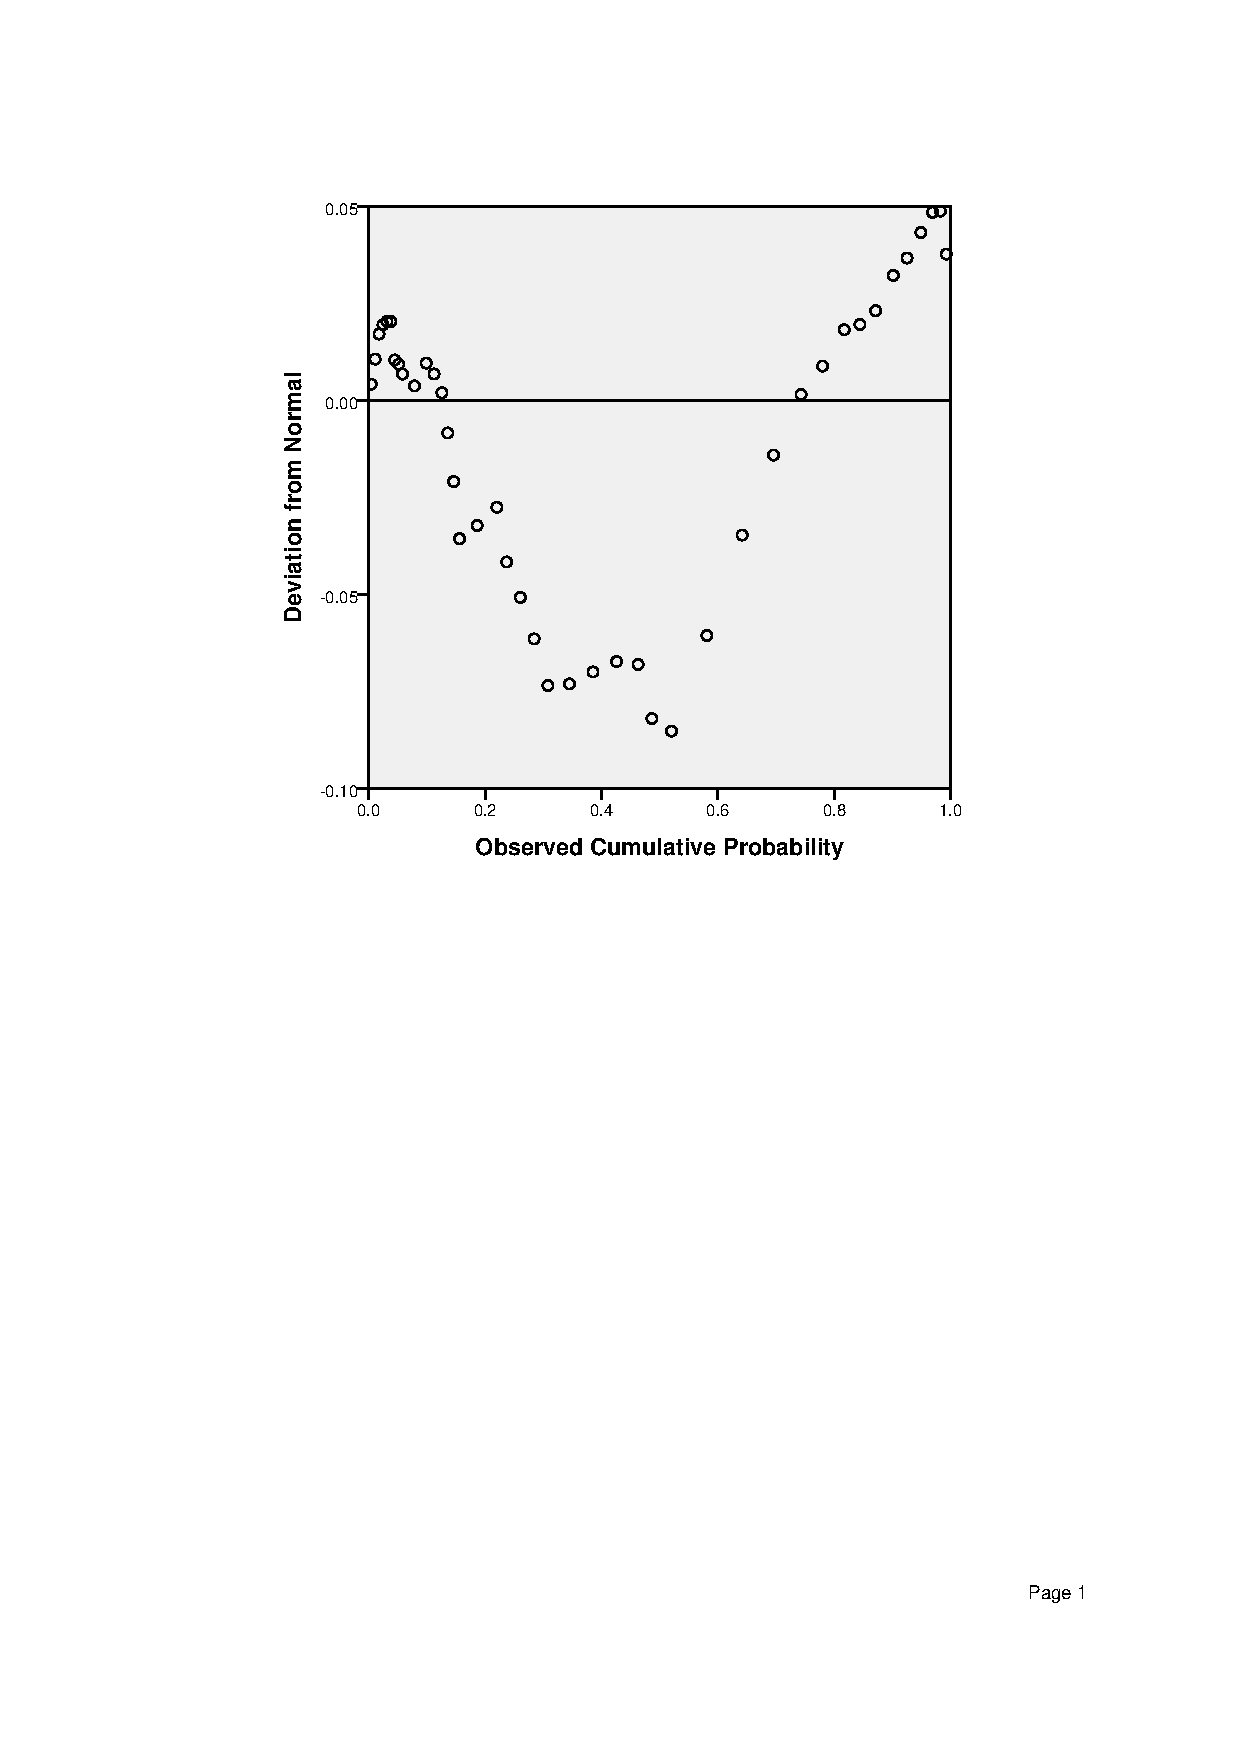
\includegraphics[width=\textwidth,
	%height=\graphdiv\textheight,
	trim={2.5cm 15cm 2.5cm 3cm},
	clip]{media/age-detrended-p-p}
%\end{minipage}
\end{figure}

\chapter{Ethical approval letter}
The letter of approval from the LSBU School of Health and Social Care Ethics
Committee is on the next page.
\pagebreak
\label{apx:ethics}
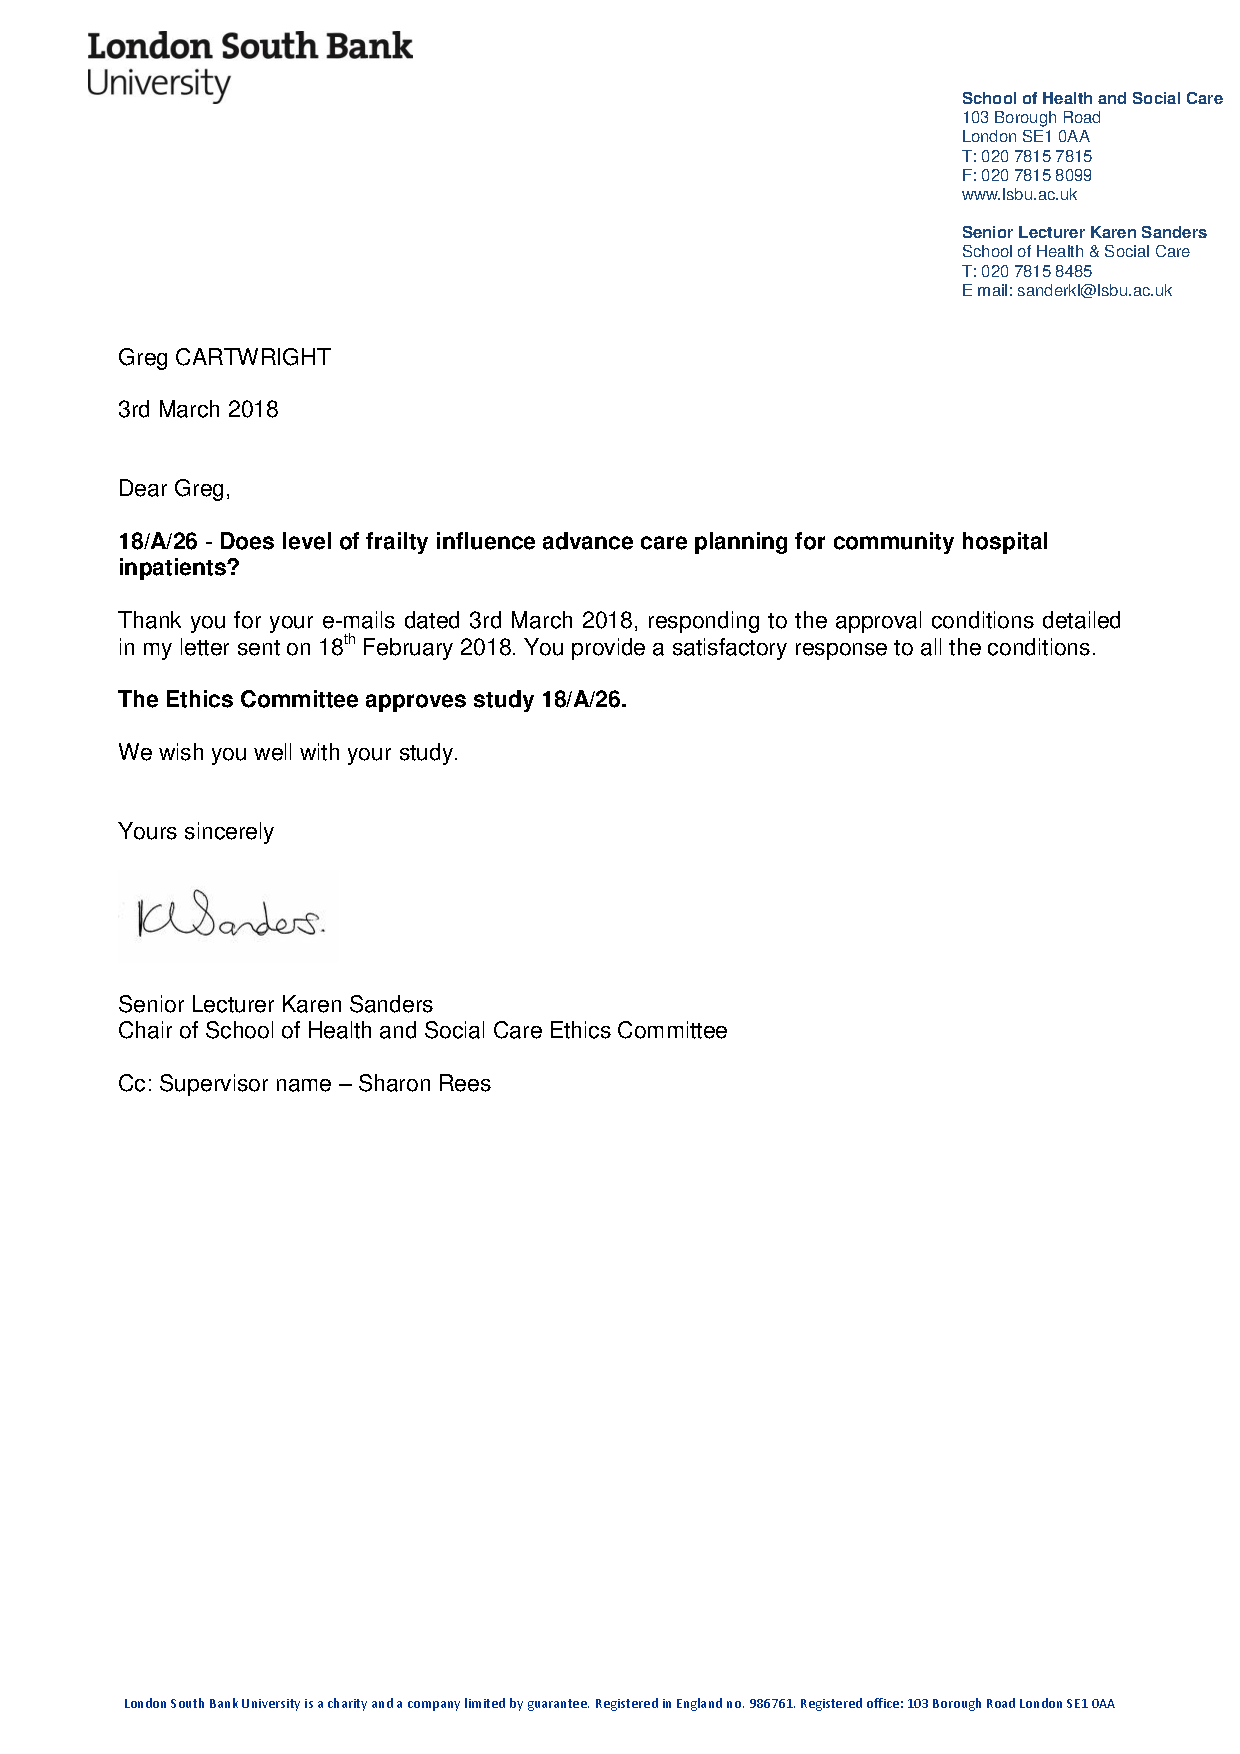
\includegraphics[width=0.8\textwidth,
	trim={1cm 0cm 1cm 0cm},
	clip]{media/final-ethics-approval}

\chapter{Raw SPSS output}
\label{apx:raw-spss}
\begin{center}
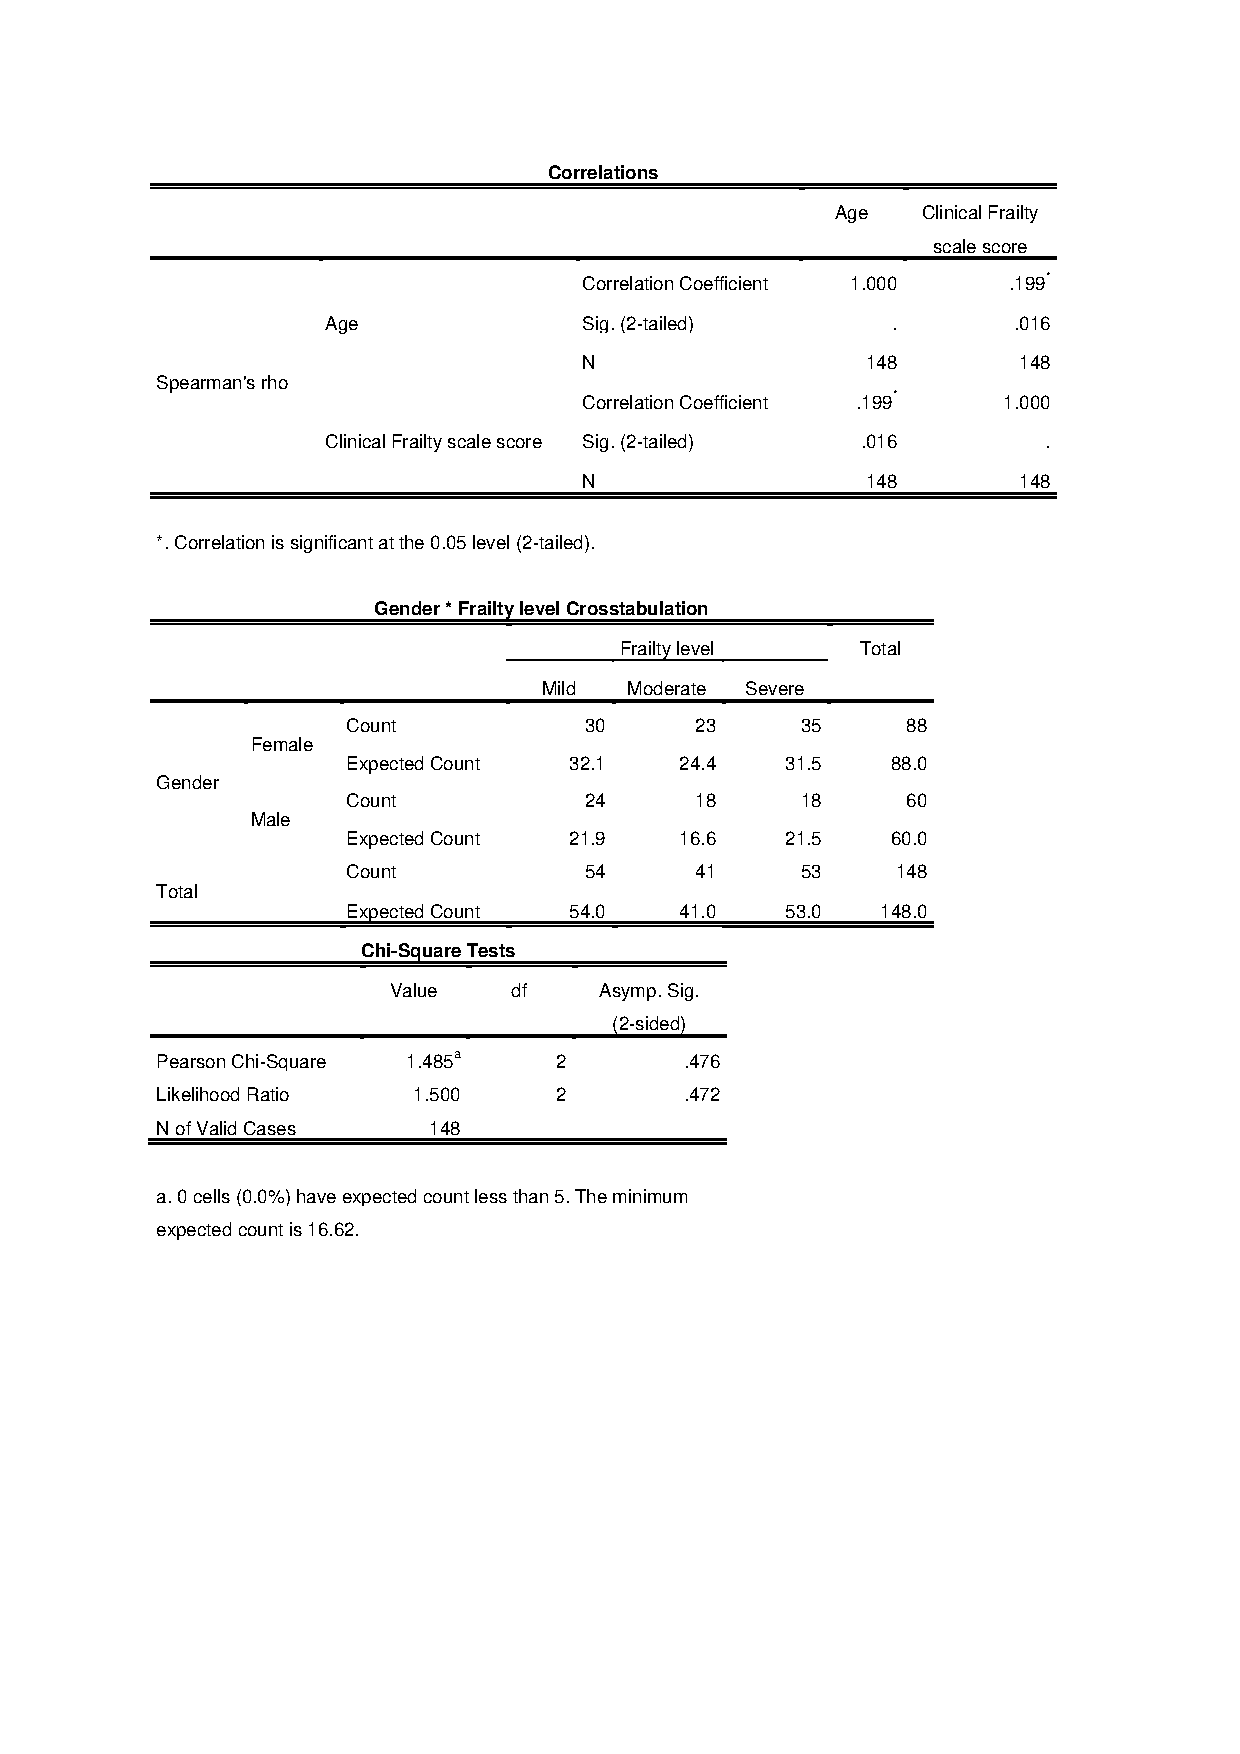
\includegraphics[width=0.7\textwidth,
	page=1,
	trim={2.5cm 8cm 2.5cm 2.5cm},
	clip]{media/raw-spss}
\end{center}
\pagebreak
\begin{center}
\includegraphics[width=0.8\textwidth,
	page=2,
	trim={2.5cm 8cm 2.5cm 2.5cm},
	clip]{media/raw-spss}
\end{center}
\pagebreak
\begin{center}
\includegraphics[width=0.8\textwidth,
	page=3,
	trim={2.5cm 8cm 2.5cm 2.5cm},
	clip]{media/raw-spss}
\end{center}

\end{document}
